\documentclass[preprint,12pt,authoryear]{elsarticle}

\usepackage{graphicx}
\usepackage{booktabs}
\usepackage{multirow}
\usepackage{amsmath,amssymb}
\usepackage{subfig}
\usepackage{url}

\journal{Computerized Medical Imaging and Graphics}

\begin{document}

\begin{frontmatter}

\title{BAMNet: Joint Aortic Root Segmentation and Landmark Localization on Intraoperative Fluoroscopy for TAVI Guidance}

\author[label1]{Nikita V. Laptev\corref{cor1}}
\ead{nikitalaptev77@gmail.com}

\author[label2]{Olga M. Gerget}
\ead{olgagerget@mail.ru}

\author[label3]{Julia K. Panteleeva}

\author[label3]{Mikhail A. Chernyavsky}

\author[label4]{Viacheslav V. Danilov}
\ead{viacheslav.v.danilov@gmail.com}

\cortext[cor1]{Corresponding author}

\address[label1]{Siberian State Medical University, 2 Moskovsky Trakt, Tomsk 634050, Russia}
\address[label2]{V.A. Trapeznikov Institute of Control Sciences of Russian Academy of Sciences, 65 Profsoyuznaya Street, Moscow 117997, Russia}
\address[label3]{Almazov National Medical Research Centre, 2 Akkuratova Street, Saint Petersburg 197341, Russia}
\address[label4]{Pompeu Fabra University, Carrer de la Merc\`{e} 12, 08002 Barcelona, Spain}

\begin{abstract}
Accurate intraoperative delineation of the aortic root and localization of key anatomical landmarks during transcatheter aortic valve implantation (TAVI) remain difficult because fluoroscopy provides low soft-tissue contrast and is frequently degraded by motion and overlap from catheters and delivery systems. This study developed and validated a multitask deep learning model for simultaneous aortic root segmentation and landmark localization on fluoroscopic images to support image-guided TAVI. A retrospective dataset of 2,925 fully anonymized fluoroscopic frames from 83 patients who underwent TAVI between 2018 and 2024 was used. Expert annotations included binary masks of the contrast-enhanced aortic root and four anatomical landmarks: two aortic annulus points (AA1, AA2) and two sinotubular junction points near the coronary ostia (STJ1, STJ2). We developed BoundaryAwareMANet (BAMNet), a multitask architecture combining an EfficientNet-V2 encoder, an MA-Net-inspired decoder, a coordinate-aware landmark head, and an auxiliary boundary-guidance pathway. Model performance was evaluated using patient-level five-fold cross-validation. Across five folds, BAMNet achieved Dice $0.916 \pm 0.011$, IoU $0.850 \pm 0.018$, and Surface Dice@4 mm $0.845 \pm 0.031$. Landmark localization reached median and mean errors of $7.64 \pm 0.33$ px and $10.02 \pm 0.17$ px. The model produced both segmentation masks and landmark coordinates in a single forward pass, maintaining real-time inference at approximately 63 FPS. Joint segmentation of the aortic root and localization of anatomical landmarks on intraoperative fluoroscopy is feasible.
\end{abstract}

\begin{keyword}
TAVI \sep aortic root segmentation \sep landmark localization \sep multitask learning \sep fluoroscopy
\end{keyword}

\end{frontmatter}

\section{Introduction}

Aortic stenosis remains one of the most common and clinically important valvular diseases in aging populations worldwide. As life expectancy increases, the number of patients with severe aortic stenosis also continues to rise. Transcatheter aortic valve implantation (TAVI) has become a major interventional treatment option in contemporary cardiology, with expanding indications in patients at intermediate and low surgical risk \citep{otto2020_guideline,vahanian2021_guidelines,leon2019_partner3}.

Despite this expansion, optimal valve positioning during deployment remains a major determinant of procedural success and long-term outcome. Suboptimal implantation depth and alignment relative to the annular plane and coronary ostia may increase the risk of paravalvular regurgitation, coronary obstruction, or conduction disturbances requiring permanent pacemaker implantation \citep{pibarot2021_pvl,jilaihawi2022_coronary,kammler2016_implantdepth}. Accurate real-time visualization is therefore central to safe guidance.

In current clinical practice, operators rely primarily on fluoroscopy, often supplemented by repeated contrast aortography to delineate the aortic root, annular plane, and coronary ostia. Fluoroscopy offers high temporal resolution, but it also suffers from low soft-tissue contrast, noise, respiratory and cardiac motion, and frequent occlusion by guidewires, catheters, and delivery systems. These limitations increase dependence on contrast administration and operator experience. Hybrid approaches based on preoperative CT and CT-fluoroscopy fusion have been explored for procedural guidance, but their accuracy may be limited by cardiorespiratory motion, deformation from stiff guidewires, and the lack of continuous real-time updating during valve deployment \citep{vernikouskaya2017_imageguidance,vernikouskaya2018_registration}.

Recent work has begun to address the segmentation task in this setting. In a prior study by our group \citep{laptev2025_aorticroot}, we performed a large-scale comparison of six modern convolutional architectures for automatic aortic root segmentation on intraoperative TAVI frames. On a dataset of 2,925 images from 83 patients with strict patient-level 5-fold cross-validation, the best single-task model, MA-Net with an EfficientNet-B4 encoder, achieved a median Dice score of 0.94 and an average symmetric surface distance (ASSD) of 4.07 mm. These results demonstrated that high-quality segmentation is feasible even under low-contrast fluoroscopic conditions. However, a segmentation mask alone is insufficient when sub-pixel landmark coordinates are needed for automated or robotic valve positioning.

The next stage in TAVI guidance is the transition toward robot-assisted and potentially autonomous delivery platforms. Early translational robotic systems are already emerging, including AI-guided positioning studies and the ongoing feasibility evaluation of the TAVIPILOT platform \citep{smits2025_autonomous,clinicaltrials_nct07152574}. Such systems require not only a contour of the aortic root, but also reliable and temporally stable localization of key landmarks, especially the two annular points (AA1 and AA2) and the two sinotubular-junction landmarks near the coronary ostia (STJ1 and STJ2).

To address this clinical and technological need, we developed BAMNet, a multitask architecture for simultaneous aortic root segmentation and precise localization of four landmarks on intraoperative fluoroscopic images. We further hypothesized that combining global contextual reasoning, coordinate-aware feature modulation, and explicit boundary-focused supervision in a unified multitask formulation would improve both segmentation quality and landmark localization performance.

\section{Materials and methods}

\subsection{Dataset and annotation protocol}

The study used intraoperative fluoroscopic images acquired during TAVI procedures in patients with severe aortic stenosis. The present work builds on a previously published dataset of intraoperative angiographic images \citep{laptev2025_dataset} and extends it with additional patients and revised annotations. The final dataset comprised 2,925 grayscale images of size $1000 \times 1000$ pixels (8-bit) obtained from 83 patients between 2018 and 2024.

The primary annotation task was binary segmentation of the aortic root. The expert mask represented the visible contour of the contrast-enhanced aortic root in the current frame. Guidewires, catheters, valve delivery system components, and other radiopaque instruments were deliberately excluded from the mask. Annotation was performed in the Supervisely web-based computer vision platform, consistent with the previous dataset release (Fig.~\ref{fig:annotation_examples}).

\begin{figure}[htbp]
\centering
\subfloat[]{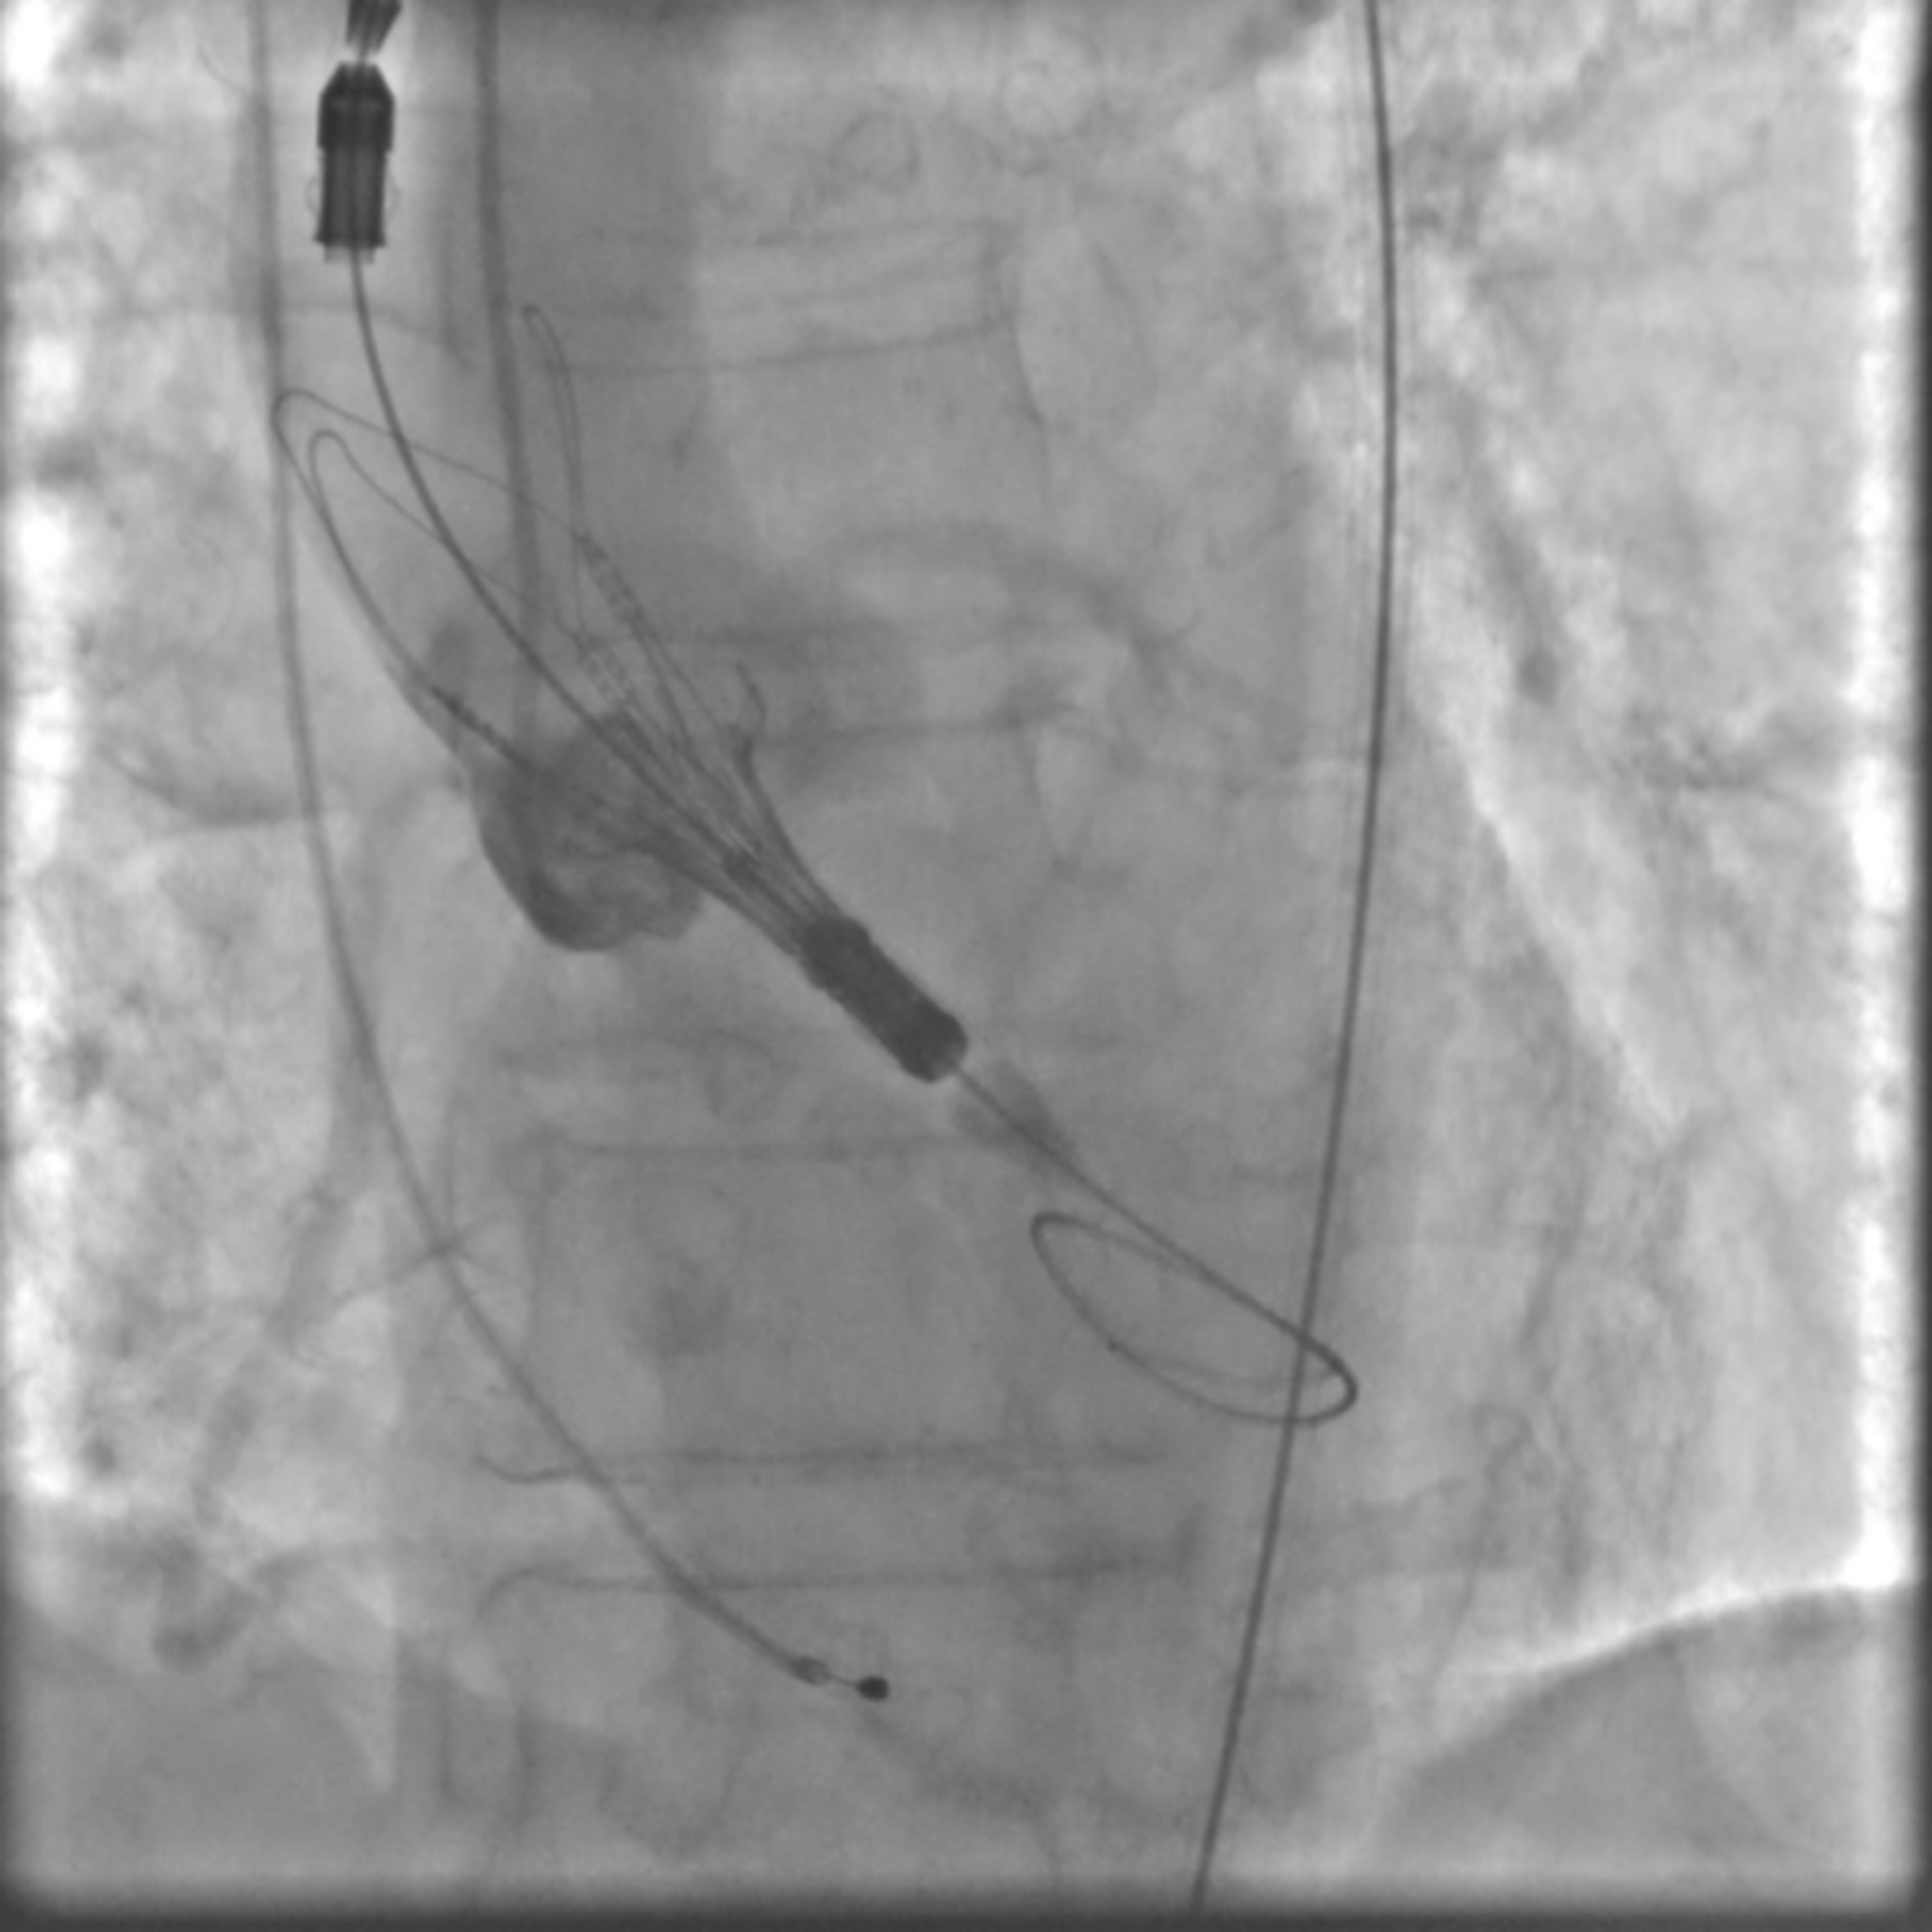
\includegraphics[width=0.48\textwidth]{figures/Figure_1a.png}}
\hfill
\subfloat[]{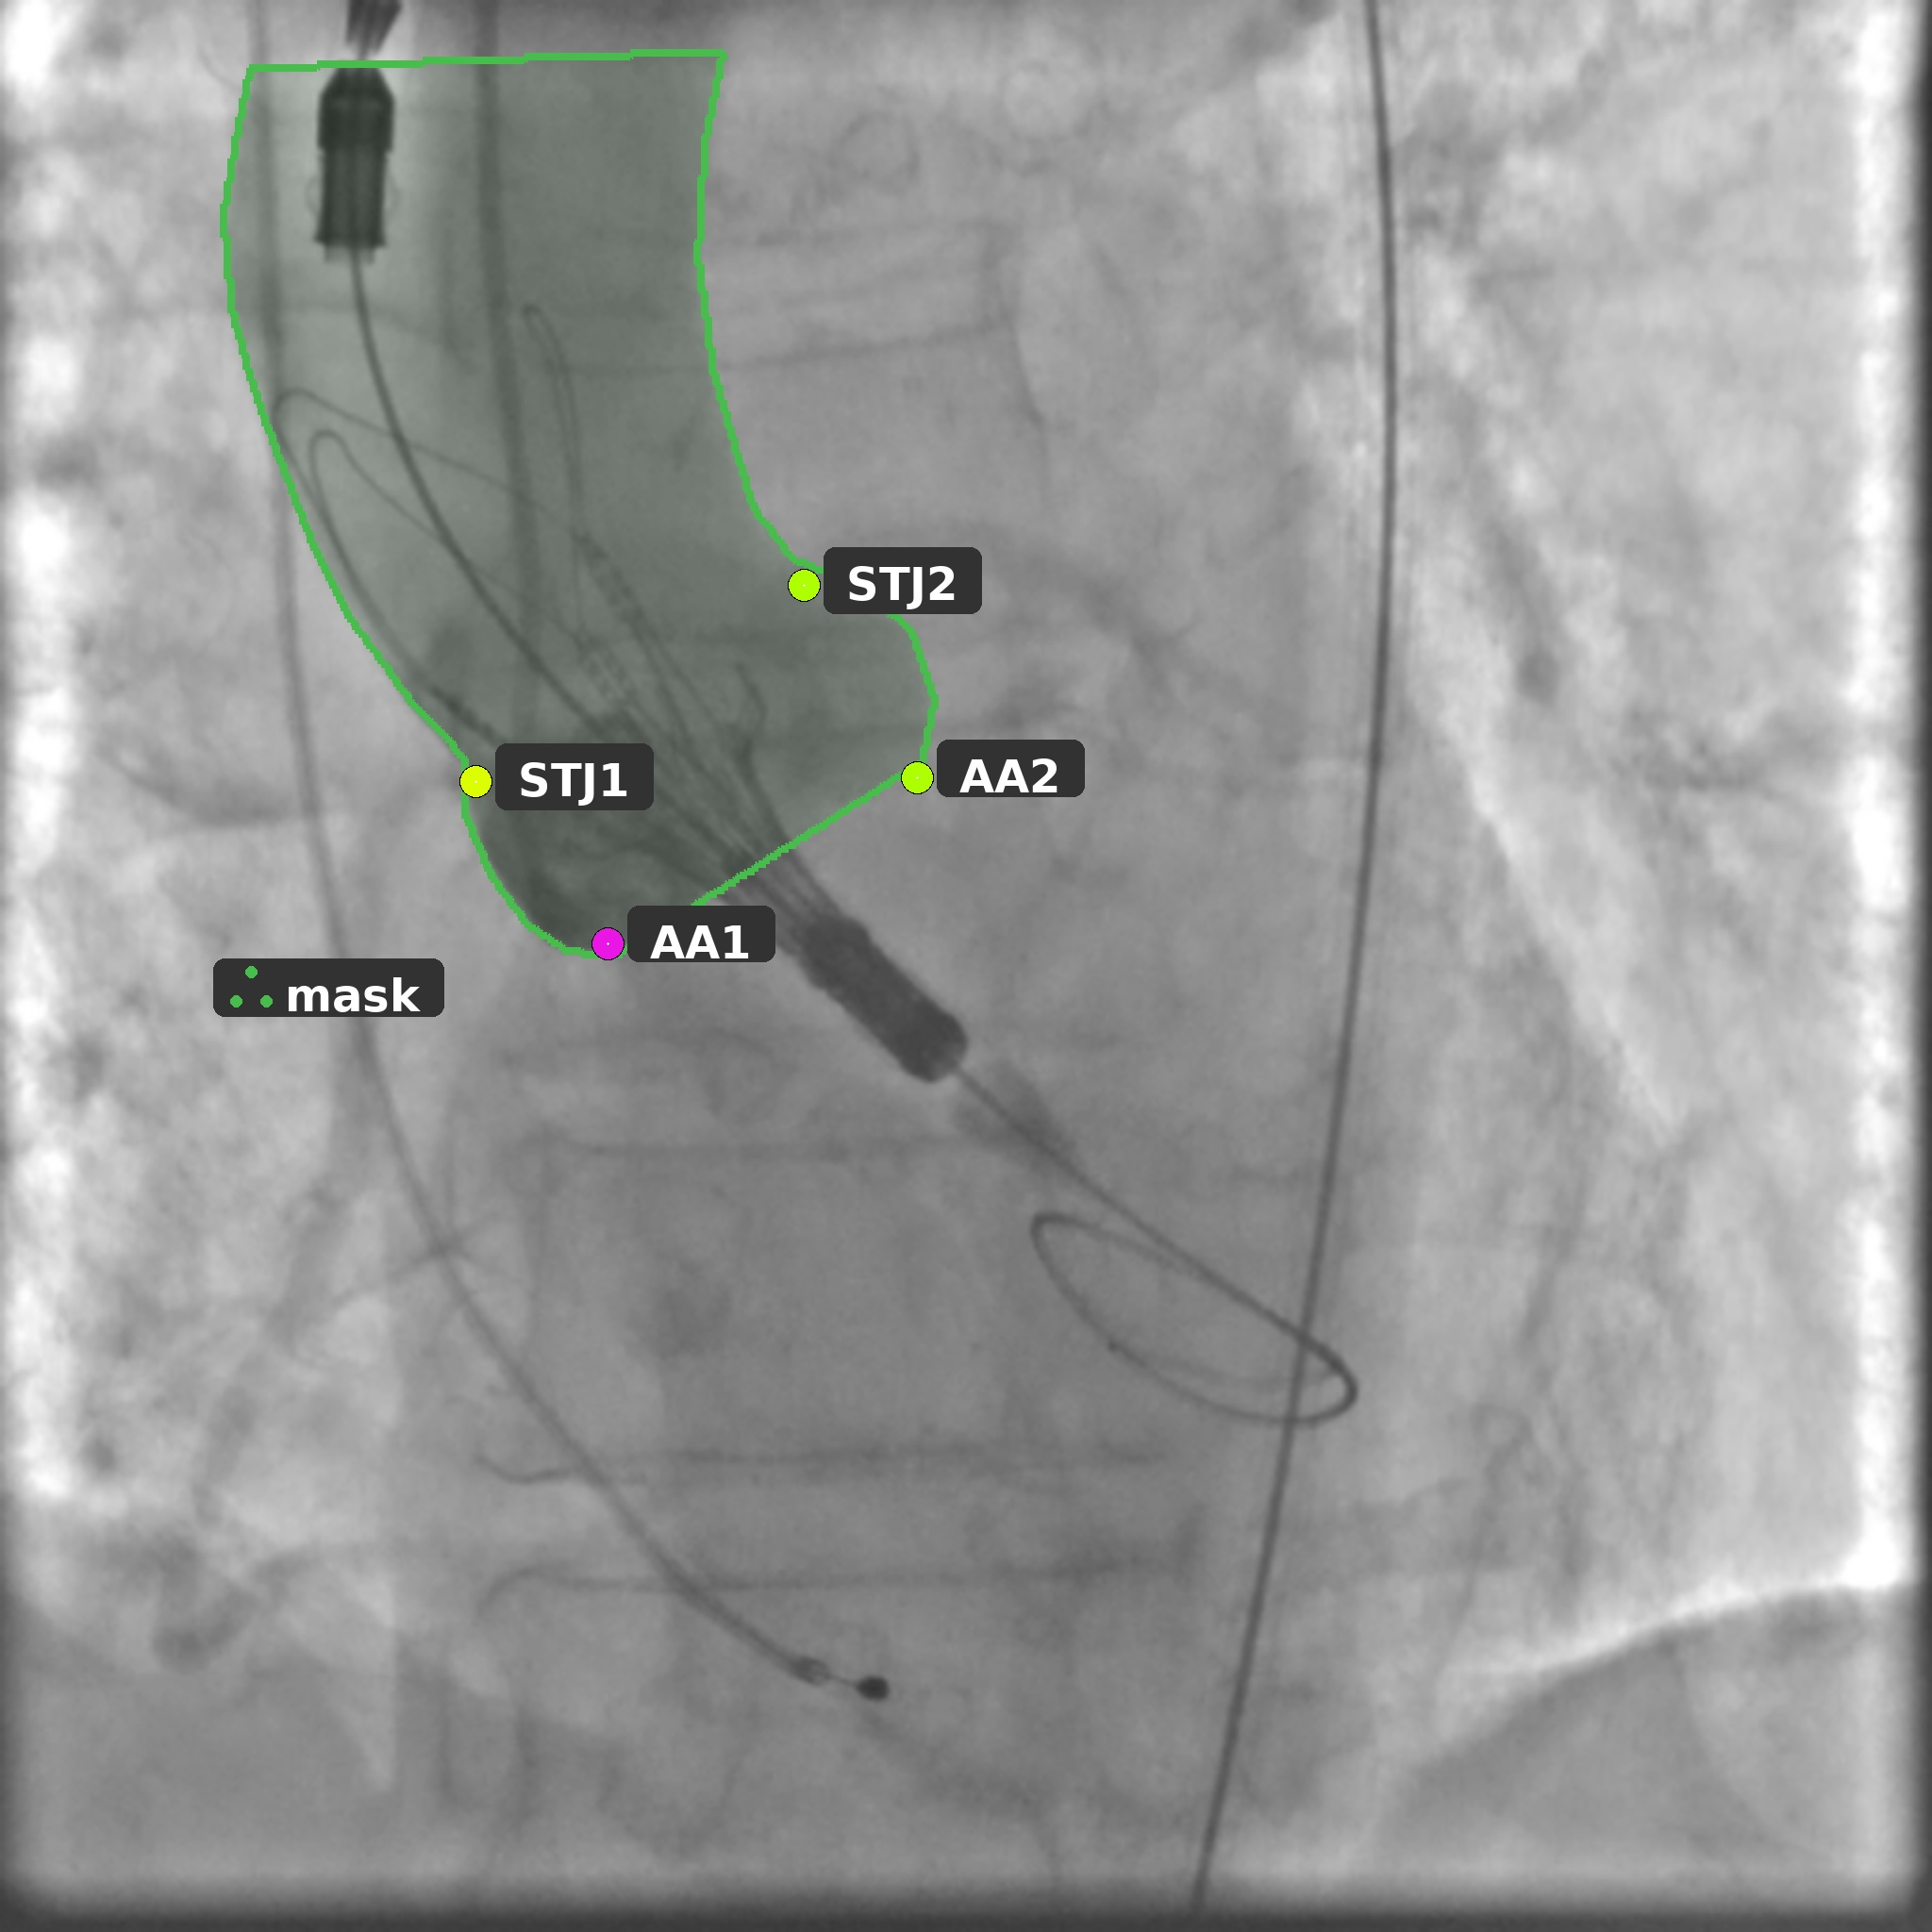
\includegraphics[width=0.48\textwidth]{figures/Figure_1b.jpeg}}\\[0.8em]
\subfloat[]{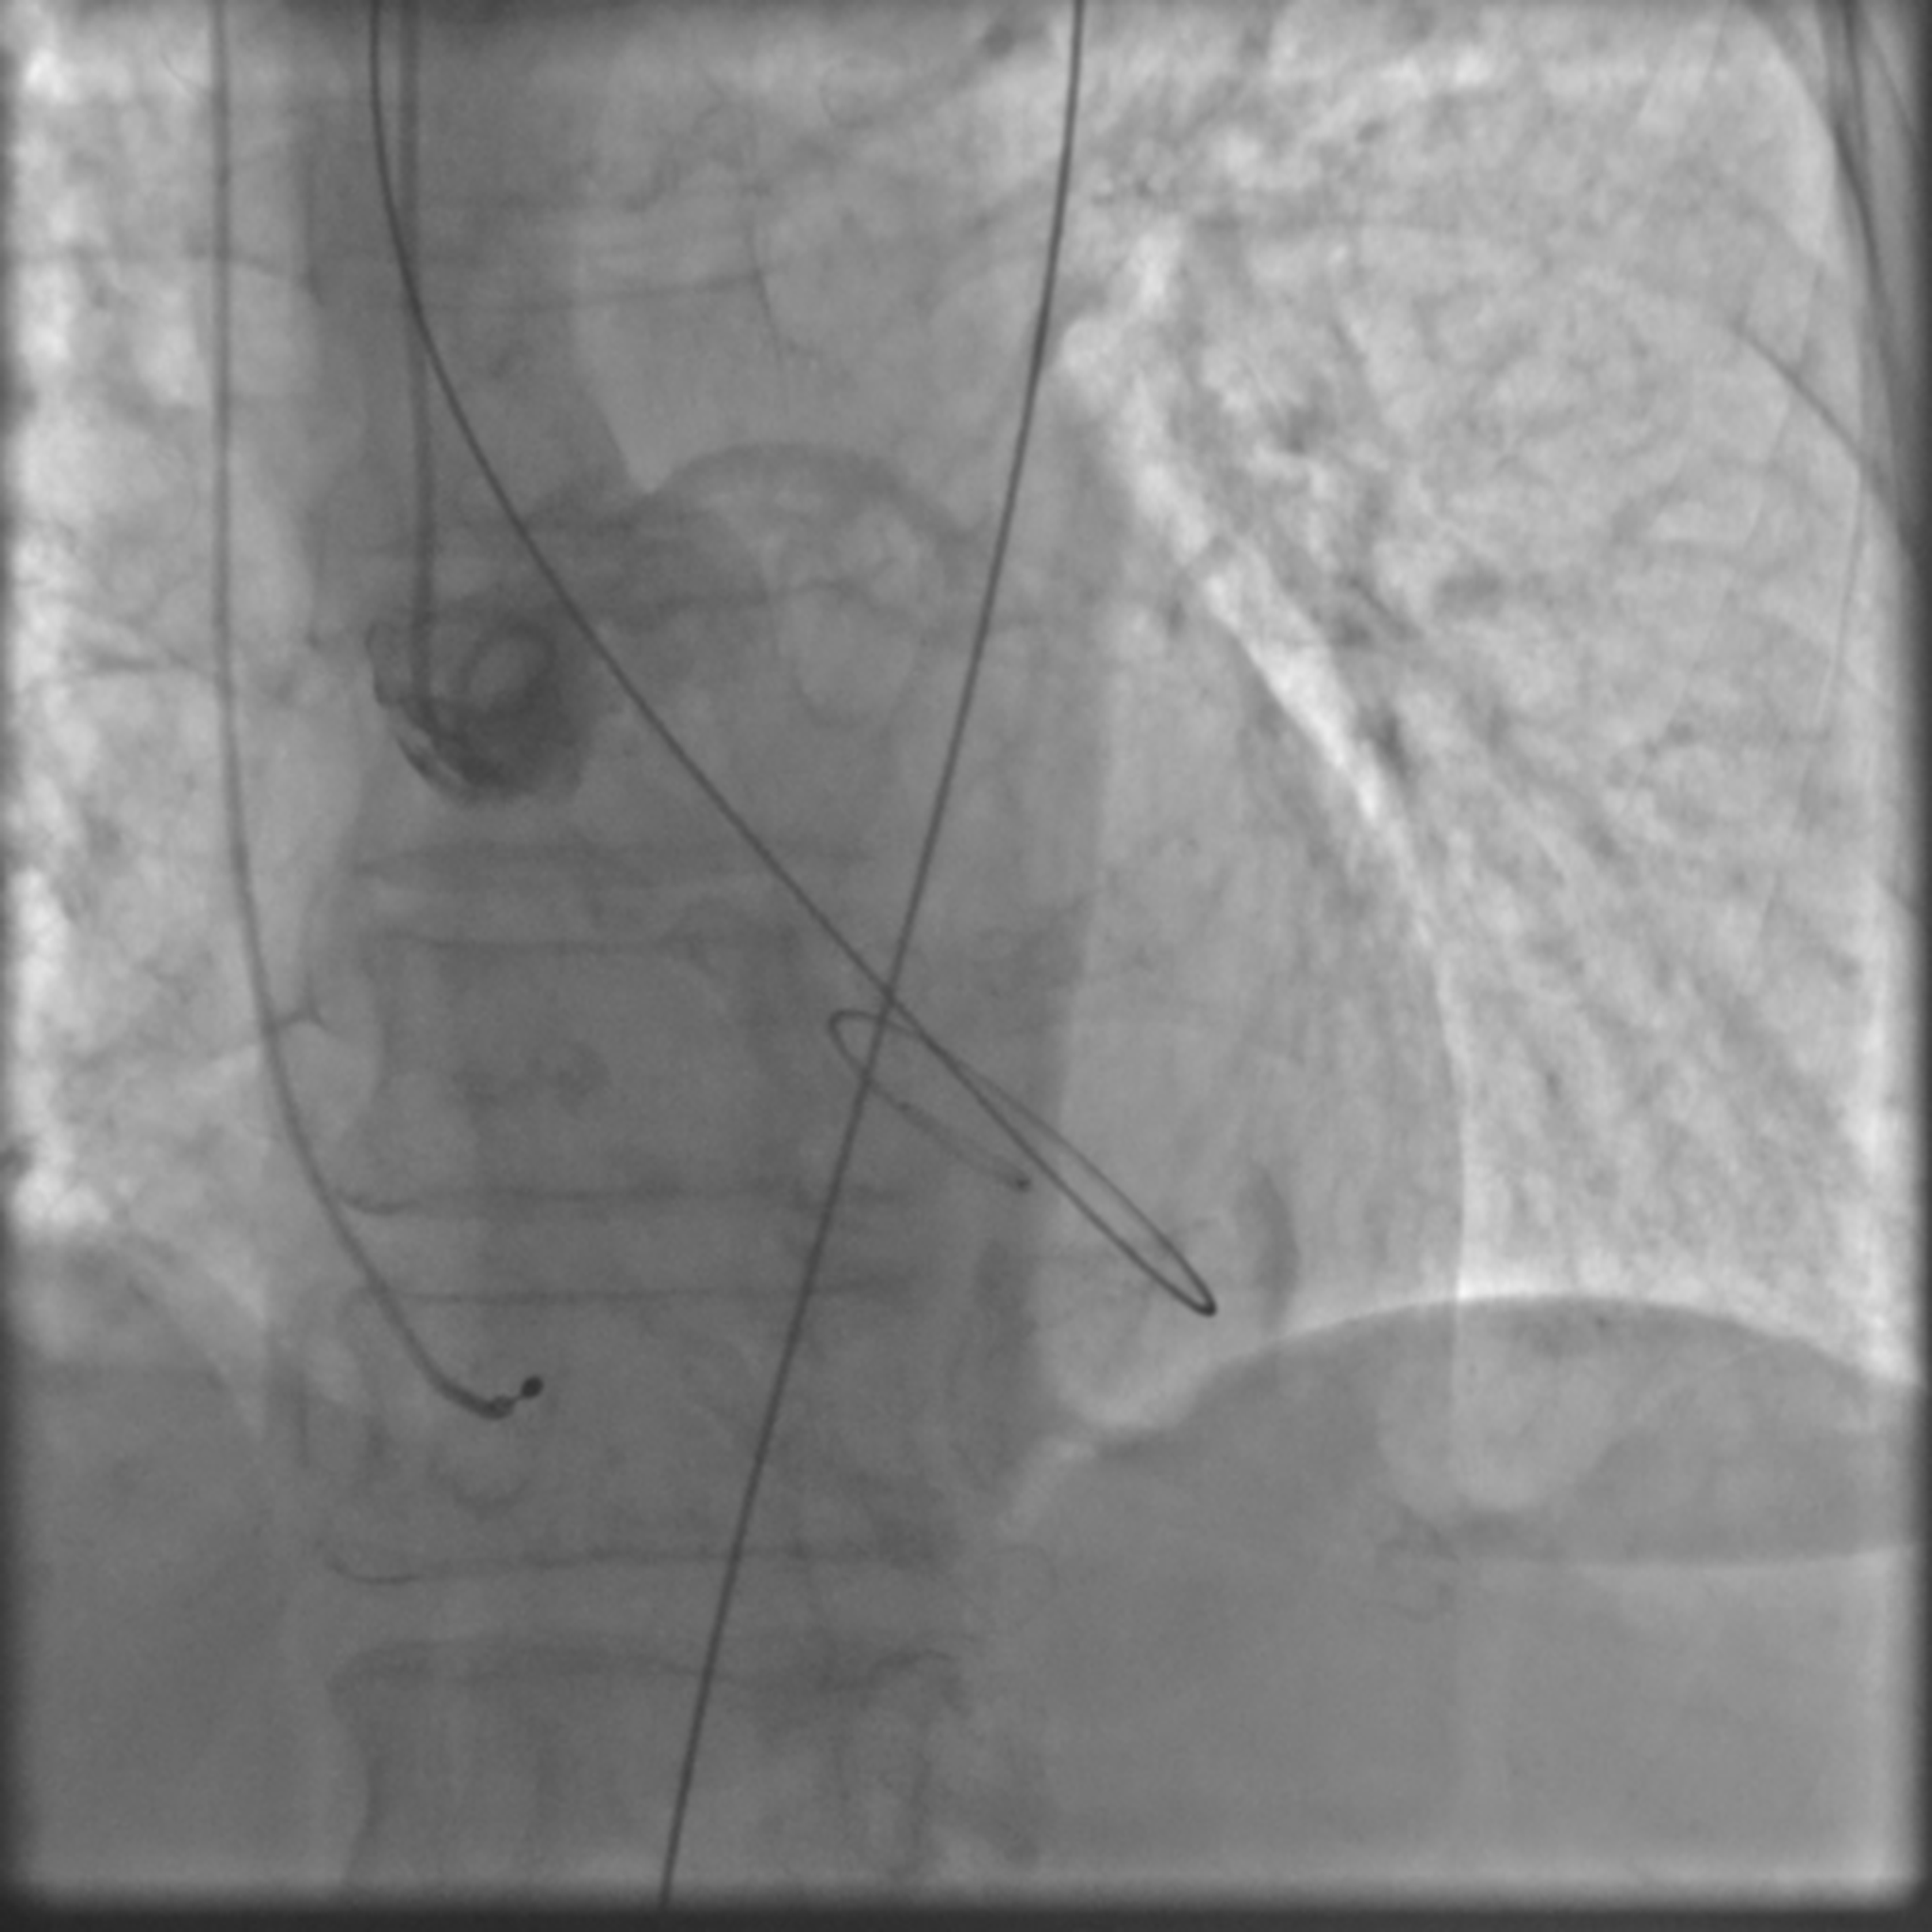
\includegraphics[width=0.48\textwidth]{figures/Figure_1c.png}}
\hfill
\subfloat[]{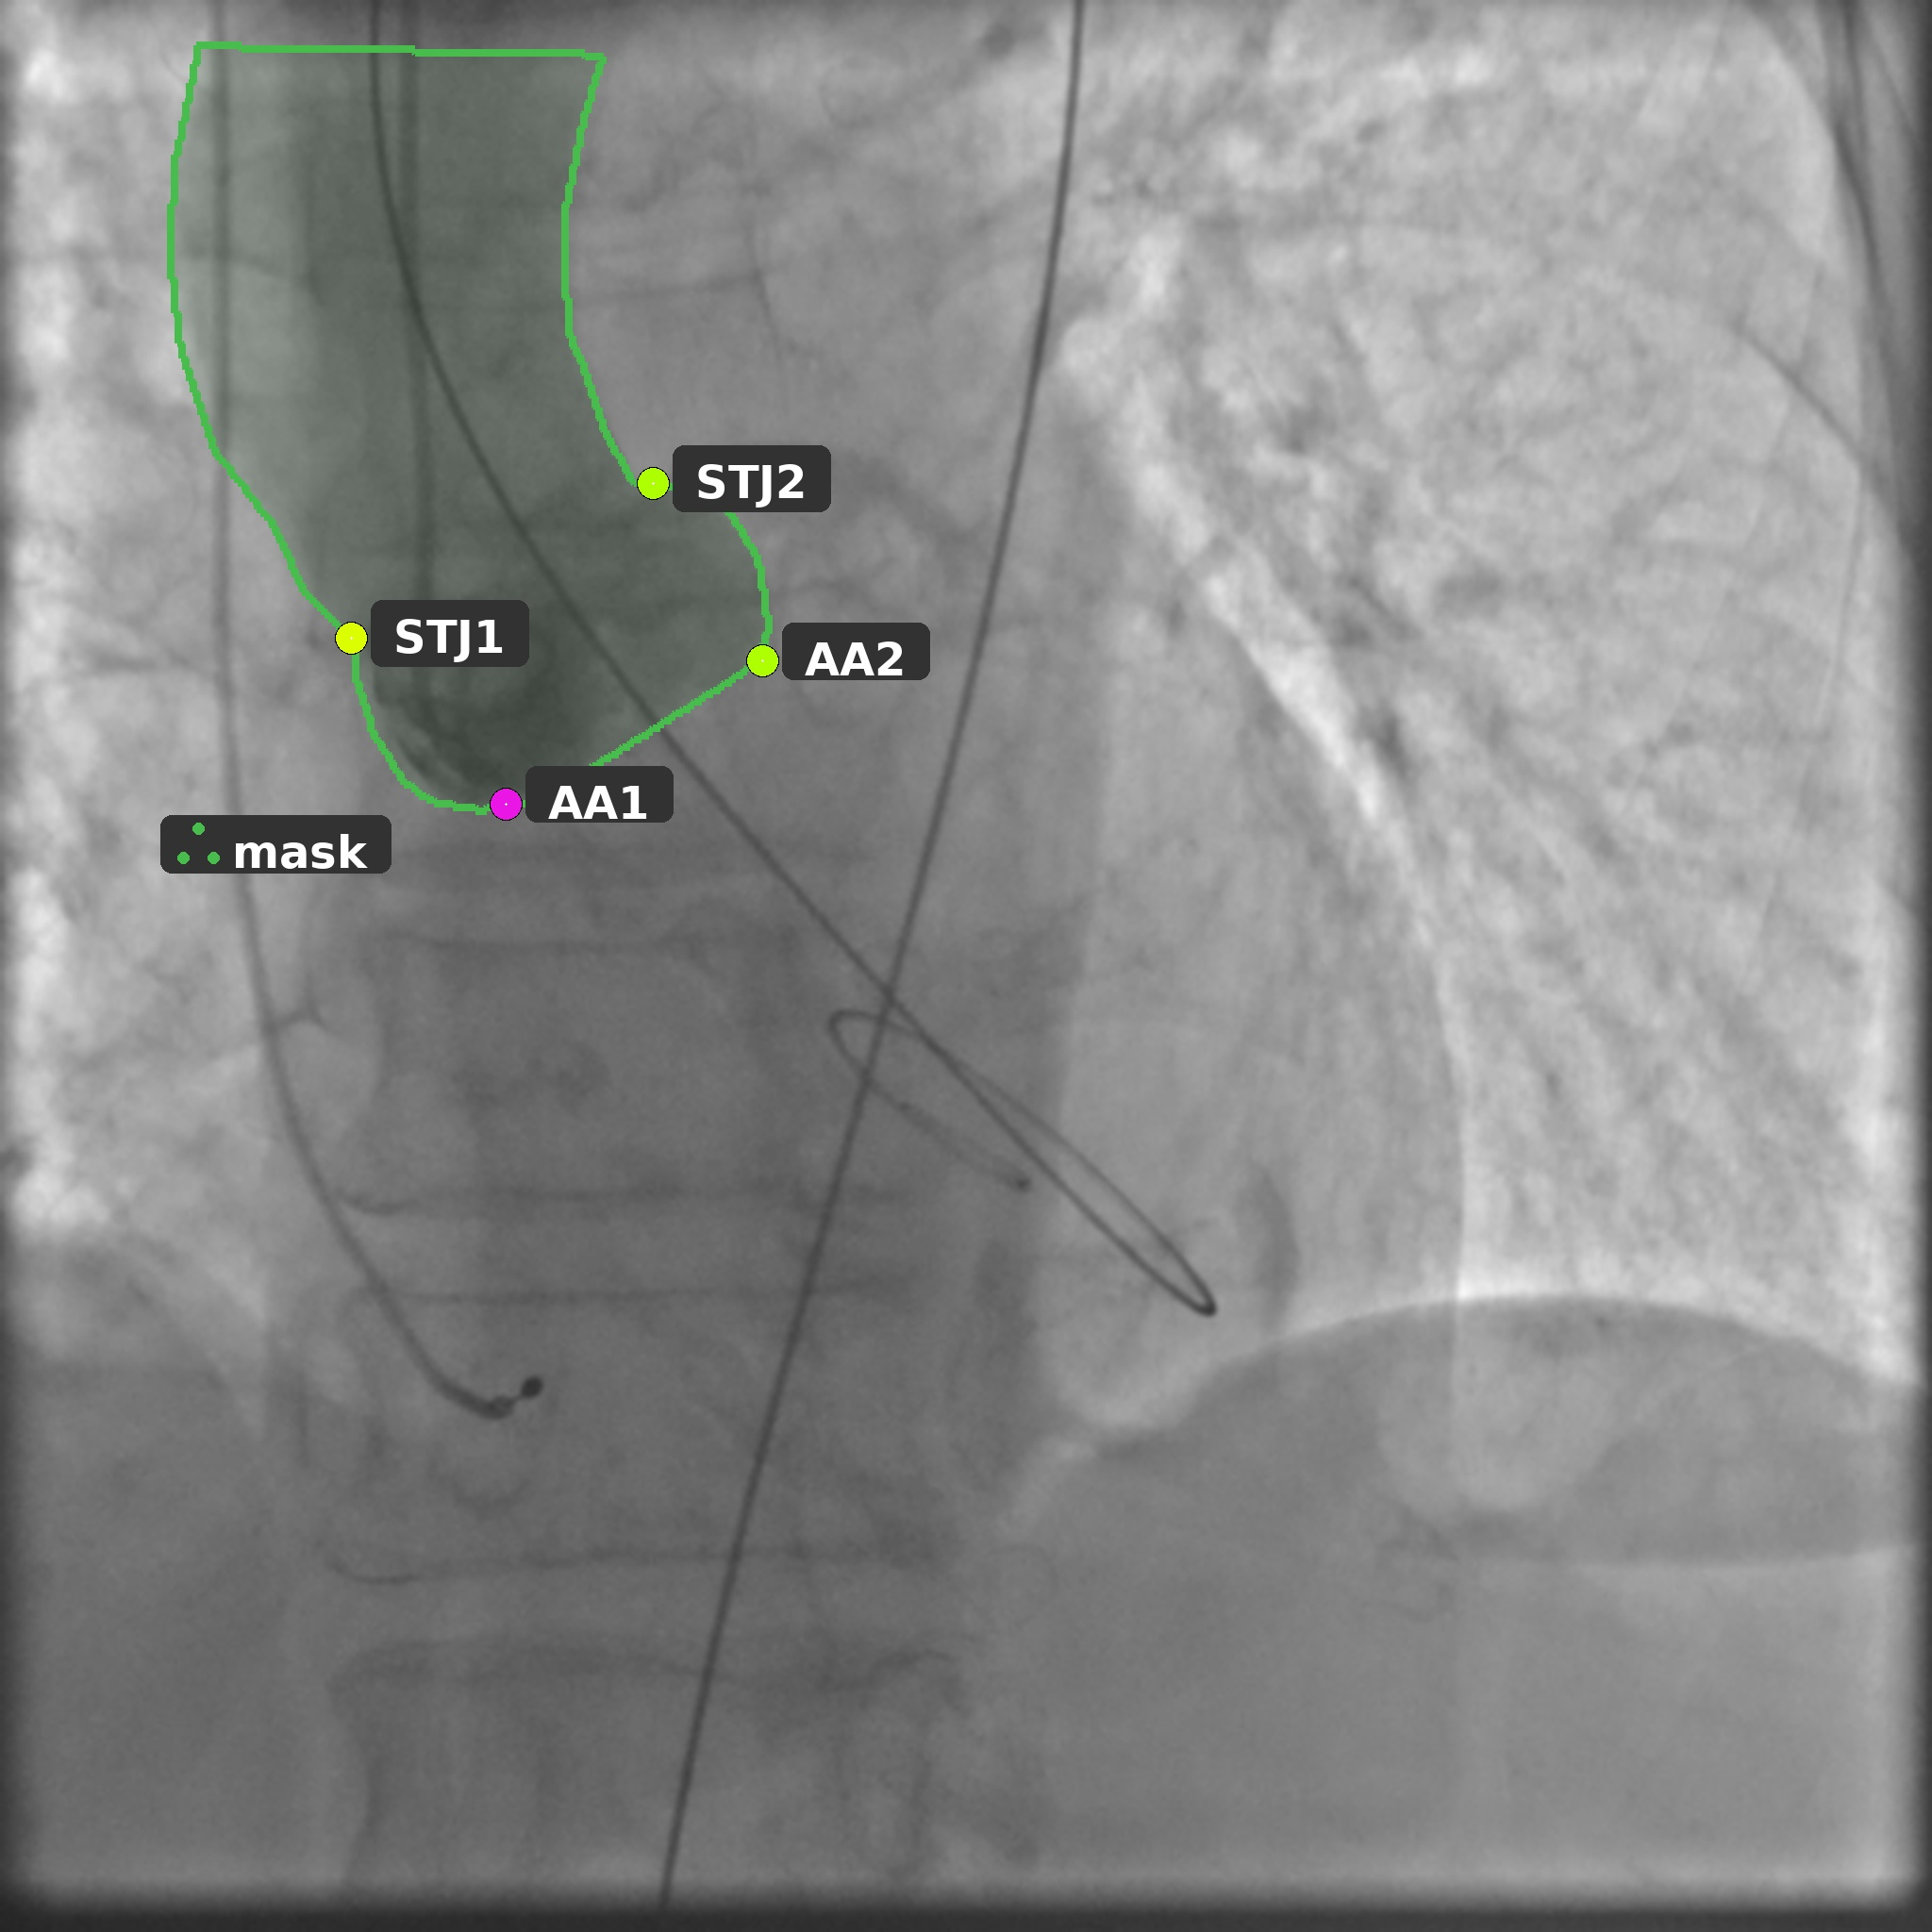
\includegraphics[width=0.48\textwidth]{figures/Figure_1d.jpeg}}
\caption{Representative fluoroscopic images (a, c) and corresponding expert annotations (b, d) illustrating the aortic root mask and four anatomical landmarks (AA1, AA2, STJ1, STJ2).}
\label{fig:annotation_examples}
\end{figure}

In addition to binary masks, each image was annotated with four key anatomical landmarks: two points on the aortic annulus (AA1 and AA2) and two landmarks near the coronary ostia at the sinotubular junction (STJ1 and STJ2). For each landmark, two-dimensional coordinates $(x,y)$ and a binary visibility flag were stored. A landmark was considered visible only when its position could be identified reliably on the current frame. When anatomy was obscured by devices, contrast opacification was insufficient, or the anatomical configuration was ambiguous, the landmark was marked as invisible.

To assess generalization properly, all experiments followed a patient-level protocol that prevented frames from the same patient from appearing in both training and validation or test subsets. Five-fold patient-level cross-validation was used throughout. In each fold, approximately 86--88\% of patients were assigned to training and 12--14\% to validation or test. Because the number of frames per patient varied, the exact image counts differed slightly across folds.

\subsection{Training strategy}

Before model input, all images were resized to a fixed resolution of $640 \times 640$ pixels. Original single-channel fluoroscopic frames were converted to a three-channel representation by channel duplication so that an ImageNet-pretrained encoder could be used. Images were then standardized with ImageNet mean and standard deviation values. Segmentation masks were resized with nearest-neighbor interpolation to preserve binary structure. Landmark coordinates were recomputed after geometric transforms and normalized to the $[0,1]$ range.

Augmentations were applied only to the training subset and were implemented with custom transformations. Their purpose was both to enlarge the effective training distribution and to regularize the model against overfitting. The augmentation pipeline included horizontal flipping with probability 0.5, accompanied by mandatory swapping of landmark pairs AA1$\leftrightarrow$AA2 and STJ1$\leftrightarrow$STJ2; affine transforms with scaling in the range 0.85--1.15, rotations within $\pm 20^{\circ}$, translations up to $\pm 8$\% along each axis, and mild shear up to $\pm 5^{\circ}$; moderate elastic deformation; contrast-limited adaptive histogram equalization-based local contrast enhancement; random brightness and contrast adjustment; gamma correction; additive Gaussian noise; Gaussian blur and motion blur; simulated illumination non-uniformity and vignetting; and coarse dropout to mimic partial occlusion by interventional tools. Vertical flipping was intentionally excluded because it is not anatomically plausible in this fluoroscopic setting. If a landmark moved outside the image after a geometric transform, its visibility flag was reset to zero.

Training was performed in PyTorch with PyTorch Lightning. AdamW was used as the optimizer with an initial learning rate of $5 \times 10^{-4}$ and weight decay of $3 \times 10^{-4}$. The learning rate was adapted with ReduceLROnPlateau using a validation balance score that combined segmentation quality and landmark localization accuracy. To stabilize optimization, several parameters were scheduled smoothly. The soft-argmax temperature increased during early epochs from $\beta=2$ to $\beta=12$, enabling a transition from smoother to more localized coordinate distributions. At the same time, the width of the Gaussian target heatmaps was gradually reduced so that training started from softer targets and then shifted toward higher spatial precision.

The contribution of the landmark branch and the influence of boundary-guided feature enhancement were also introduced progressively to avoid early optimization instability. In later epochs, the weight of the point-related loss component was reduced to improve the balance between segmentation quality and landmark localization.

\subsection{Proposed multitask architecture}

BoundaryAwareMANet (BAMNet) was designed as a single multitask network for simultaneous dense segmentation of the aortic root and localization of anatomical landmarks. Both tasks are solved in one forward pass, which is important for intraoperative deployment under real-time latency constraints.

The model is built on an ImageNet-pretrained EfficientNet-V2 encoder that extracts features at multiple spatial scales. These features are fused in a decoder inspired by U-Net and MA-Net so that the network can combine global anatomical context with local contour details. At low-resolution decoder levels, additional spatial attention is applied to improve reconstruction of the continuous aortic root contour in difficult frames affected by low contrast, noise, motion, and device overlap.

The segmentation branch produces two outputs:
\begin{enumerate}
\item binary segmentation logits for the aortic root;
\item an intermediate high-resolution feature representation that is reused by the landmark branch.
\end{enumerate}

The landmark branch receives fused features from the deepest encoder stage and the segmentation pathway. It consists of local convolutional processing and a Coordinate Attention module that preserves vertical and horizontal positional structure. The branch predicts landmark heatmaps, while a separate auxiliary boundary head operating on segmentation features produces a boundary-weight map. Boundary guidance is implemented by projecting segmentation features and injecting them into the landmark branch during training.

This design allows the model to exploit both global root morphology and local contour geometry when localizing landmarks. The complete architecture is shown in Fig.~\ref{fig:bamnet_architecture}.

\begin{figure}[htbp]
\centering
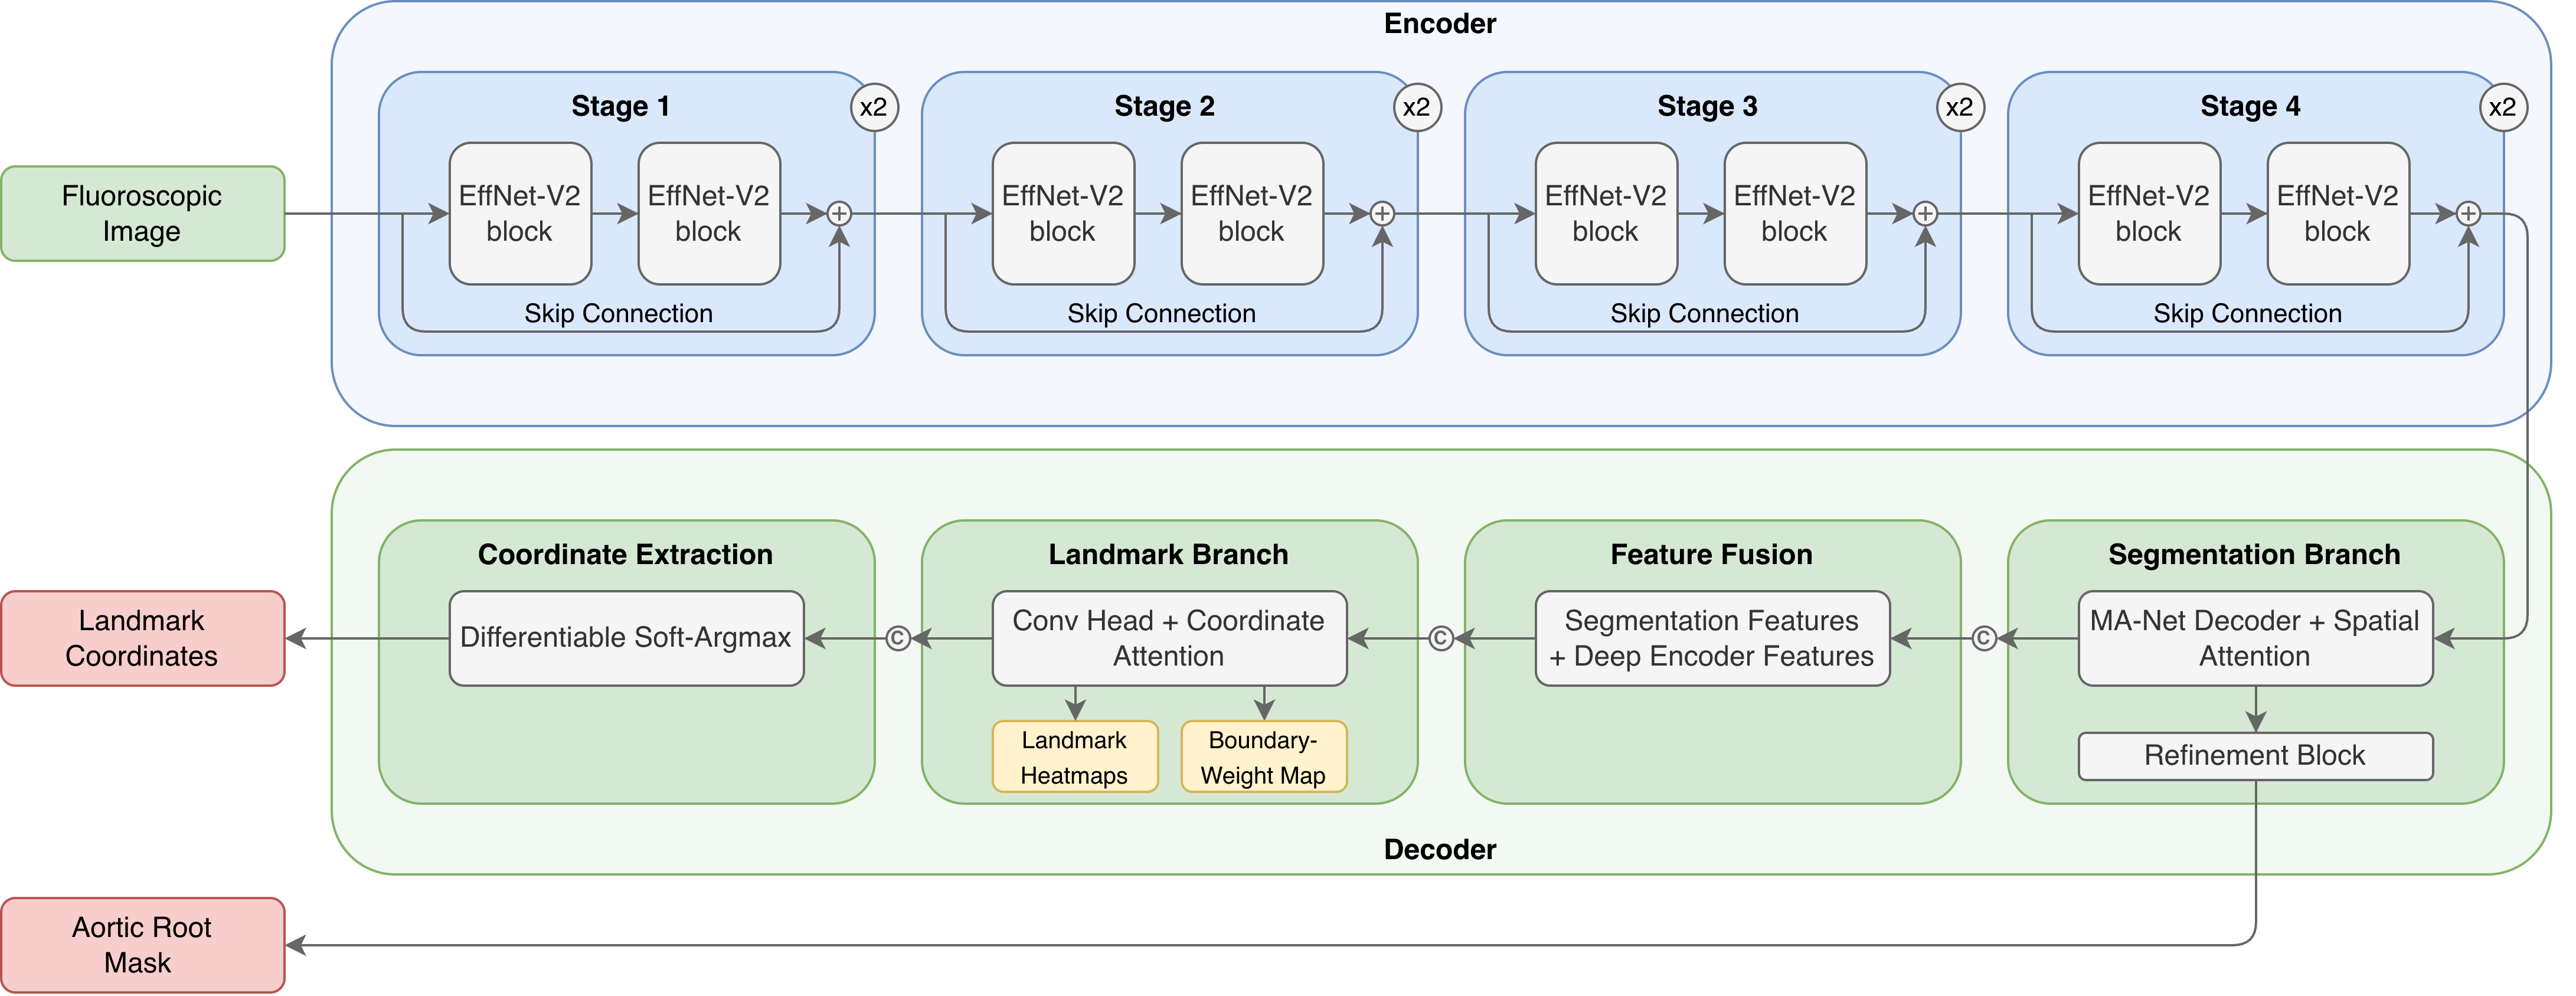
\includegraphics[width=\textwidth]{figures/Figure_2.png}
\caption{Overview of the proposed BoundaryAwareMANet (BAMNet) architecture for joint aortic root segmentation and anatomical landmark localization on fluoroscopic images. The network combines an EfficientNet-V2 encoder, a segmentation-oriented decoder, a dedicated landmark branch with Coordinate Attention, and an auxiliary boundary pathway used for boundary-guided supervision.}
\label{fig:bamnet_architecture}
\end{figure}

\subsection{Landmark coordinate extraction}

Landmark coordinates were estimated directly from predicted heatmaps using differentiable soft-argmax, which preserved gradient flow and enabled end-to-end training. For the $k$-th landmark, the pixel probability at location $(i,j)$ was defined as
\begin{equation}
P_{ij}^{(k)}=
\frac{\exp\left(\beta H_{ij}^{(k)}\right)}
{\sum\limits_{m,n}\exp\left(\beta H_{mn}^{(k)}\right)},
\end{equation}
where $H_{ij}^{(k)}$ is the heatmap logit and $\beta$ is the temperature parameter. The landmark coordinates were then computed as expectations:
\begin{equation}
\hat{x}_k=\sum\limits_{i,j} j\,P_{ij}^{(k)}, \qquad
\hat{y}_k=\sum\limits_{i,j} i\,P_{ij}^{(k)}.
\end{equation}

This formulation provides continuous, fully differentiable coordinate estimates without a separate offset-refinement stage. In addition, segmentation features were projected into the landmark branch to softly emphasize anatomically informative regions during training.

\subsection{Target generation}

To train the landmark branch, Gaussian target heatmaps were generated from expert landmark coordinates. For landmark $k$, the target heatmap was defined as
\begin{equation}
G_k(i,j)=
\exp\left(
-\frac{(i-y_k)^2+(j-x_k)^2}{2\sigma^2}
\right),
\end{equation}
where $(x_k,y_k)$ denotes the ground-truth landmark position and $\sigma$ controls the spatial width of the Gaussian target. Heatmaps were set to zero for invisible landmarks.

For the boundary branch, a separate target map was generated from the expert segmentation mask. After smoothing the mask, a Sobel-like gradient response was computed and normalized. This target explicitly emphasized the contour of the aortic root and served as an additional supervision signal.

\subsection{Loss functions}

The total loss was defined as a weighted sum of segmentation, landmark, and boundary components:
\begin{equation}
\mathcal{L}_{total} =
w_{bce}\mathcal{L}_{bce} +
w_{dice}\mathcal{L}_{dice} +
w_{pts}\mathcal{L}_{pts} +
w_{bnd}\mathcal{L}_{bnd}.
\end{equation}
In the baseline configuration, the weights were set to
\begin{equation}
w_{bce}=1.0,\qquad
w_{dice}=1.0,\qquad
w_{pts}=0.5,\qquad
w_{bnd}=10.0.
\end{equation}

Segmentation was optimized with binary cross-entropy with logits and soft Dice loss. Landmark supervision consisted of a focal heatmap term together with a coordinate regression term:
\begin{equation}
\mathcal{L}_{coord} =
\frac{1}{\sum_k v_k}
\sum_{k=1}^{4}
v_k
\sqrt{
(\hat{x}_k-x_k)^2+(\hat{y}_k-y_k)^2+\varepsilon
},
\end{equation}
where $v_k$ is the visibility flag for landmark $k$ and $\varepsilon$ is a small constant for numerical stability. The coordinate error was computed only for visible landmarks so that the model was not penalized for frames in which anatomy could not be localized reliably.

The boundary branch was trained with Smooth L1 loss between the predicted boundary map and the target map derived from the expert segmentation mask. This term improved boundary fidelity and promoted more stable landmark localization near anatomically meaningful contours.

\subsection{Evaluation metrics}

Segmentation performance was assessed with the Dice coefficient and Intersection over Union (IoU). The Dice coefficient was defined as
\begin{equation}
\mathrm{Dice} = \frac{2|P \cap G|}{|P| + |G|},
\end{equation}
where $P$ is the set of predicted mask pixels and $G$ is the set of ground-truth mask pixels. Surface Dice was used as an additional contour-sensitive metric.

Landmark localization was evaluated with mean Euclidean error, median Euclidean error, and PCK@r (percentage of correct keypoints) under several error thresholds. PCK@r was defined as
\begin{equation}
\mathrm{PCK}@r = \frac{1}{N}\sum_{k=1}^{N}\mathbb{I}(d_k \leq r),
\end{equation}
where $d_k$ is the Euclidean error for landmark $k$ and $\mathbb{I}$ is the indicator function. During training, the primary point metric was mean Euclidean error over visible landmarks, whereas the final analysis also included median error, PCK, and landmark-specific performance for AA1, AA2, STJ1, and STJ2. A combined validation score that balanced segmentation quality and landmark localization error was also monitored. In the cross-validation analysis (Section~\ref{subsec:crossval}), localization errors are reported in pixels at the model input resolution of $640 \times 640$. In the baseline comparison (Section~\ref{subsec:baseline_results}), errors are converted to millimeters using the known pixel spacing of each fluoroscopic acquisition.

\section{Results}

\subsection{Comparison with baseline models}
\label{subsec:baseline_results}

BAMNet delivered the most balanced performance among the evaluated methods by combining high-quality aortic root segmentation with accurate landmark localization in a single inference pass. This joint output is particularly attractive for intraoperative overlay generation and for integration into navigation or robotic positioning systems.

Table~\ref{tab:seg_baselines} summarizes the comparison with segmentation-oriented baselines. In terms of absolute segmentation metrics, the strongest result in this table was achieved by Swin-Unet, with Dice 0.91 and IoU 0.83. However, its inference speed was only about 2 FPS, which substantially limits practical deployment in real-time intraoperative navigation. BAMNet remained slightly below the best single-task segmentation baseline in these metrics, but preserved competitive segmentation quality while simultaneously solving landmark localization and providing substantially higher throughput (63 FPS). Compared with the MA-Net variant shown in the table, BAMNet demonstrated slightly higher Dice, IoU, and Surface Dice@4 mm together with better boundary agreement in terms of 95th-percentile Hausdorff distance (HD95) and ASSD. Relative to YOLO-seg-26m, BAMNet showed similar Dice and IoU, but stronger Surface Dice@4 mm and noticeably better boundary-sensitive metrics. Our previous publication \citep{laptev2025_aorticroot} provides additional context for interpreting these results, as it includes a broader comparison of convolutional aortic-root segmentation architectures on intraoperative TAVI frames.

\begin{table}[htbp]
\caption{Comparison of BAMNet with segmentation baselines. Evaluated on fold-1 fixed hold-out test set.}
\label{tab:seg_baselines}
\centering
\resizebox{\textwidth}{!}{%
\begin{tabular}{lcccccc}
\toprule
Model & Dice & IoU & Surface Dice@4 mm & HD95 (mm) & ASSD (mm) & FPS \\
\midrule
Swin-Unet & \textbf{0.91} & \textbf{0.83} & \textbf{0.89} & \textbf{8.17} & \textbf{1.95} & 2 \\
YOLO-seg-26l & 0.87 & 0.78 & 0.73 & 55.02 & 8.88 & 25 \\
YOLO-seg-26m & 0.90 & 0.82 & 0.81 & 19.88 & 3.86 & 27 \\
MA-Net & 0.90 & 0.82 & 0.81 & 10.27 & 2.63 & \textbf{101} \\
\textbf{BAMNet} & 0.90 & 0.82 & 0.81 & 9.62 & 2.57 & 63 \\
\bottomrule
\end{tabular}}
\end{table}

Table~\ref{tab:landmark_baselines} compares BAMNet with detection-only and keypoint-only approaches. Among single-task keypoint models, the strongest result was achieved by YOLO-keypoints-26m, with a mean localization error of 3.48 mm and a median error of 2.66 mm. BAMNet reduced the mean localization error to 3.22 mm while maintaining a comparable median error of 2.57 mm and simultaneously producing a full segmentation mask. The best median error in the table was obtained by RT-DETR (2.47 mm). BAMNet, however, achieved the lowest angle error, the lowest length error, and the highest inference speed among all evaluated methods. Taken together, these results indicate that BAMNet offers the most balanced combination of localization accuracy, geometric consistency, and computational efficiency for intraoperative use.

\begin{table}[htbp]
\caption{Comparison of BAMNet with landmark localization baselines. Evaluated on fold-1 fixed hold-out test set.}
\label{tab:landmark_baselines}
\centering
\resizebox{\textwidth}{!}{%
\begin{tabular}{lcccccc}
\toprule
Model & Mean err. (mm) & Median err. (mm) & Angle err. (deg) & Midpoint offset (mm) & Length err. (mm) & FPS \\
\midrule
YOLO-detect-26l & 8.32 & 2.71 & 9.45 & 3.29 & 3.31 & 29 \\
YOLO-detect-26m & 7.99 & 2.69 & 12.43 & 5.54 & 7.10 & 35 \\
RT-DETR & 7.84 & \textbf{2.47} & 5.84 & 2.39 & 3.92 & 24 \\
YOLO-keypoints-26l & 8.87 & 3.64 & 9.32 & 4.20 & 4.76 & 30 \\
YOLO-keypoints-26m & 3.48 & 2.66 & 5.26 & \textbf{1.83} & 3.03 & 34 \\
\textbf{BAMNet} & \textbf{3.22} & 2.57 & \textbf{4.62} & 2.02 & \textbf{2.43} & \textbf{63} \\
\bottomrule
\end{tabular}}
\end{table}

\subsection{Qualitative visualization of BAMNet outputs}

Representative BAMNet outputs on fluoroscopic frames are shown in Fig.~\ref{fig:bamnet_qualitative}. In both examples, the model simultaneously recovers the aortic root contour and provides a geometrically consistent set of landmarks and derived guidance primitives. The semi-transparent mask follows the visible root anatomy despite low soft-tissue contrast and overlap by interventional devices, while the predicted landmarks define the annular and sinotubular reference lines. From these landmarks, the overlay further visualizes the estimated aortic axis and the predicted implantation zone, which are directly relevant for intraoperative valve positioning.

These examples highlight an important practical feature of the proposed multitask formulation: BAMNet produces not only a segmentation mask, but also a clinically interpretable geometric overlay that can support visual guidance during TAVI. In this sense, the network output is already close to the type of augmented fluoroscopic display required for navigation assistance and future semi-automated deployment systems.

\begin{figure}[htbp]
\centering
\subfloat[]{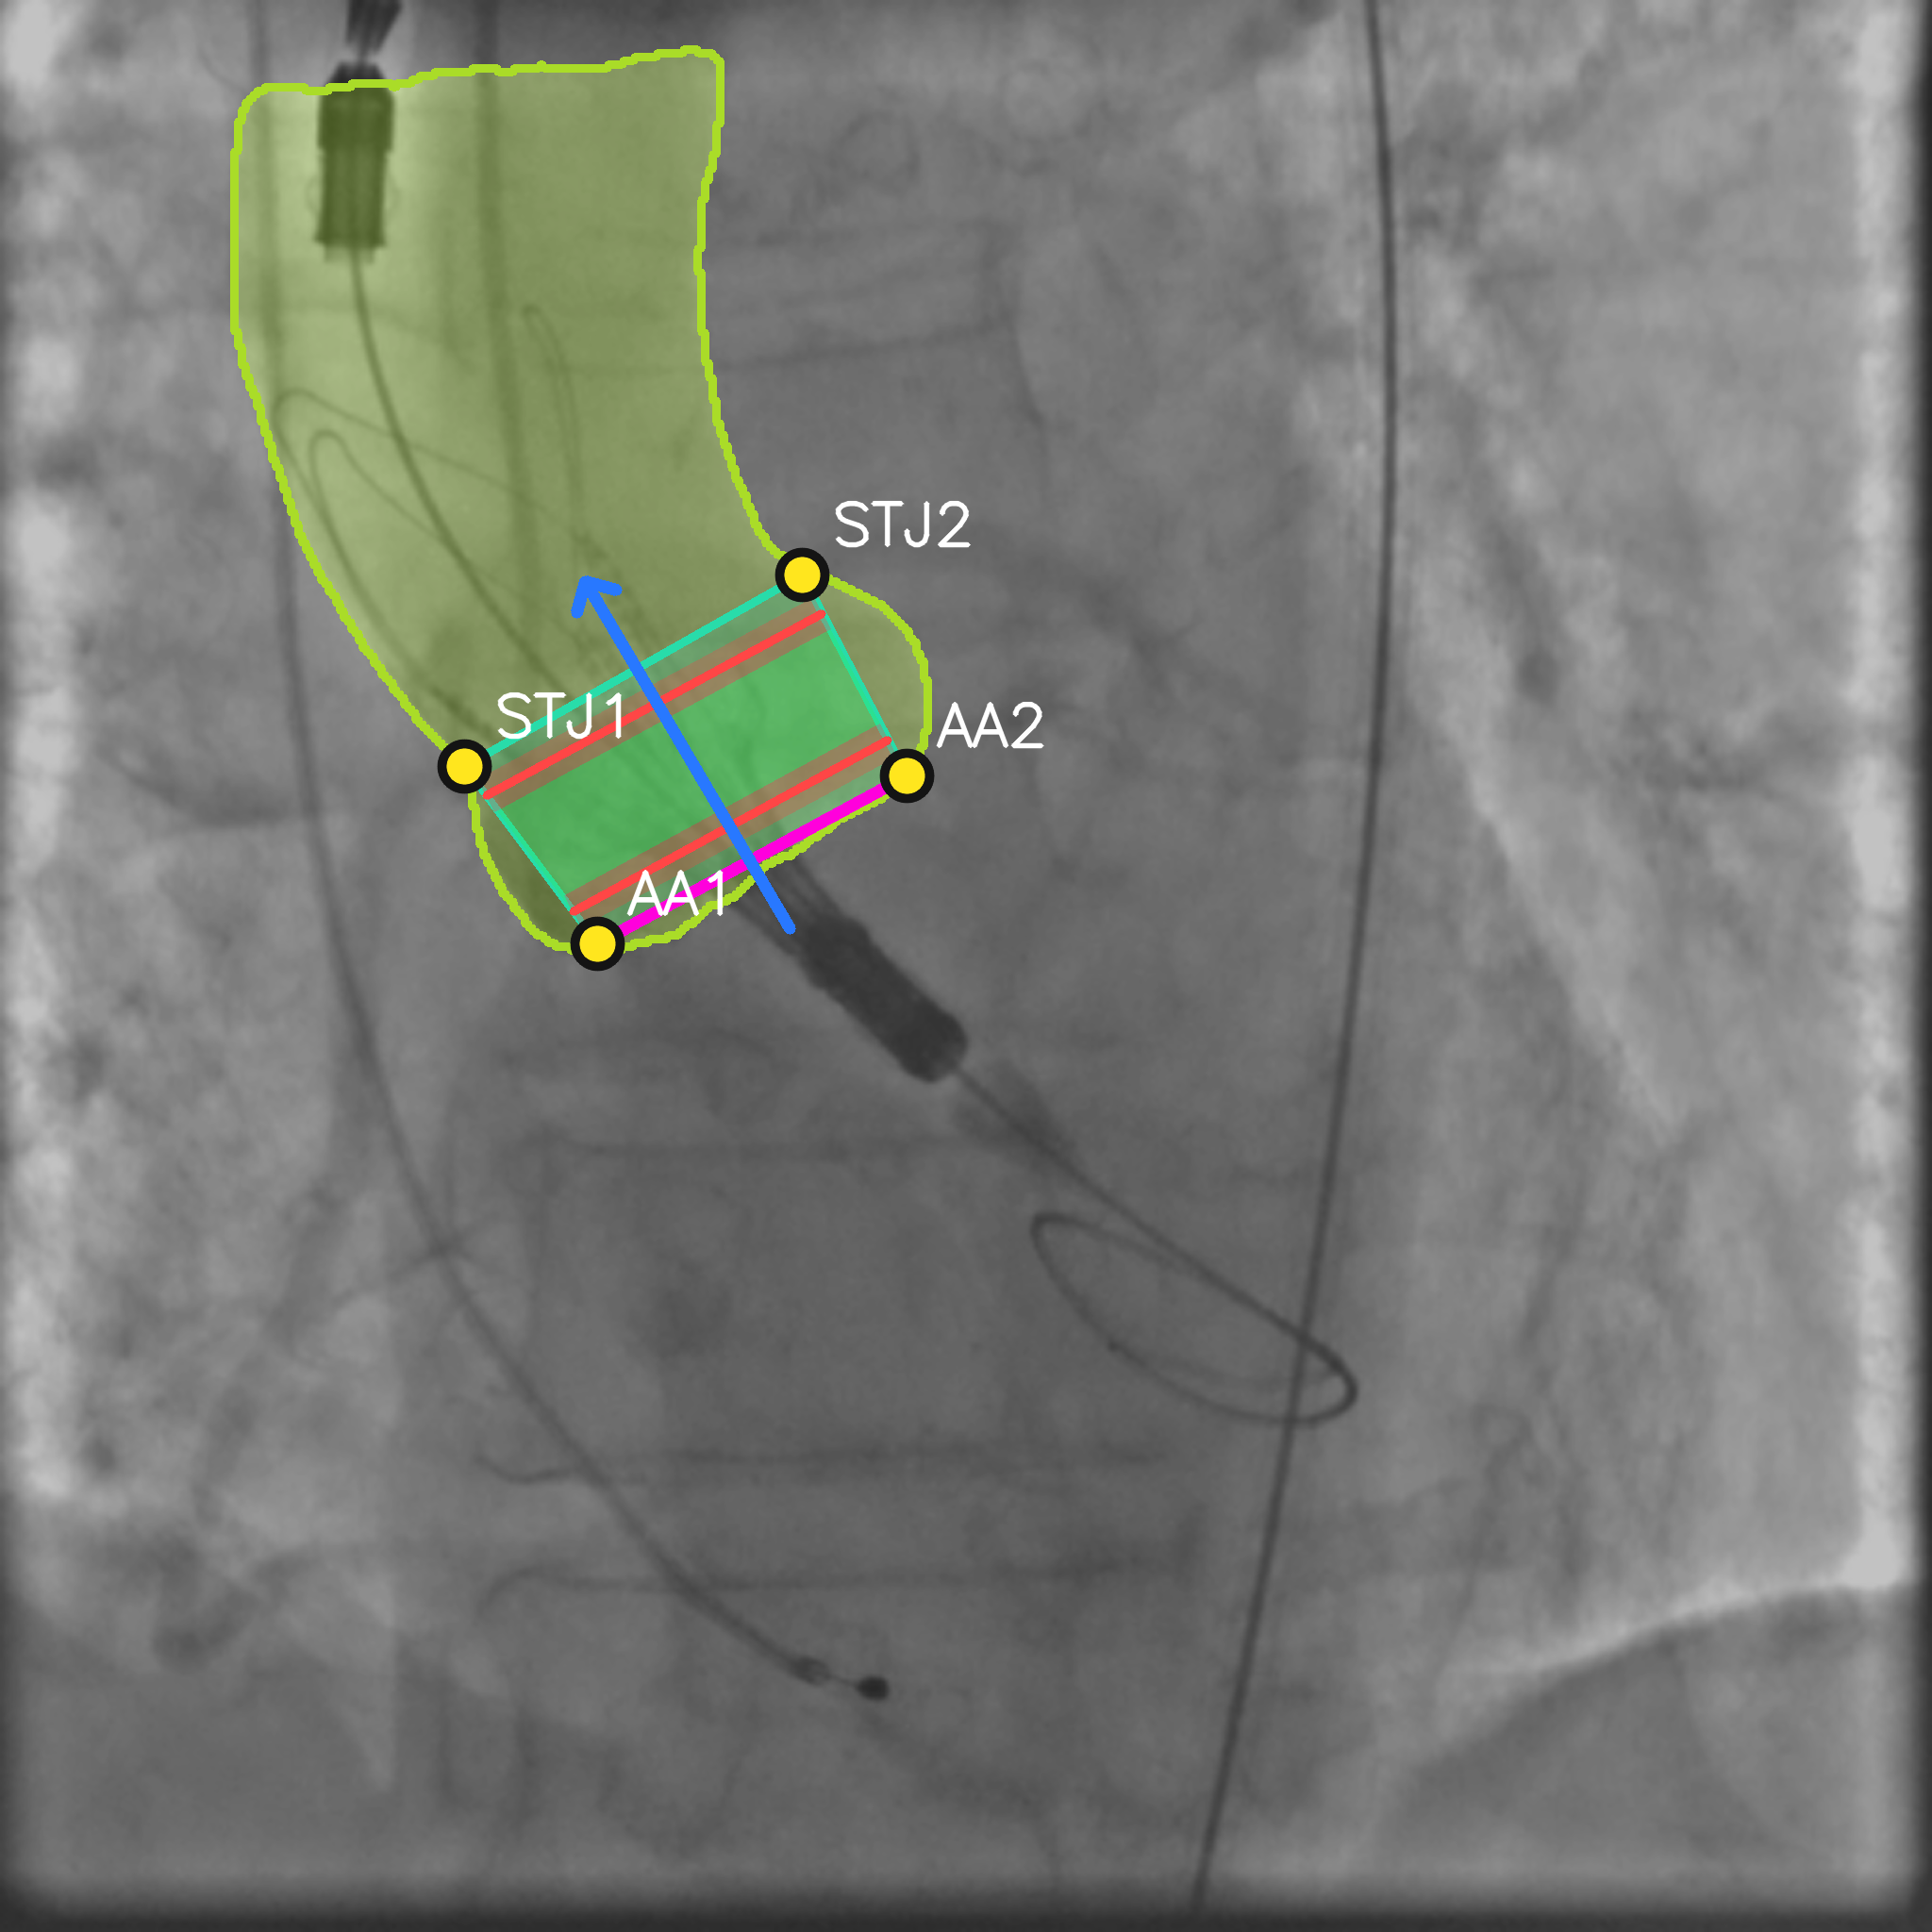
\includegraphics[width=0.48\textwidth]{figures/Figure_3a.png}}
\hfill
\subfloat[]{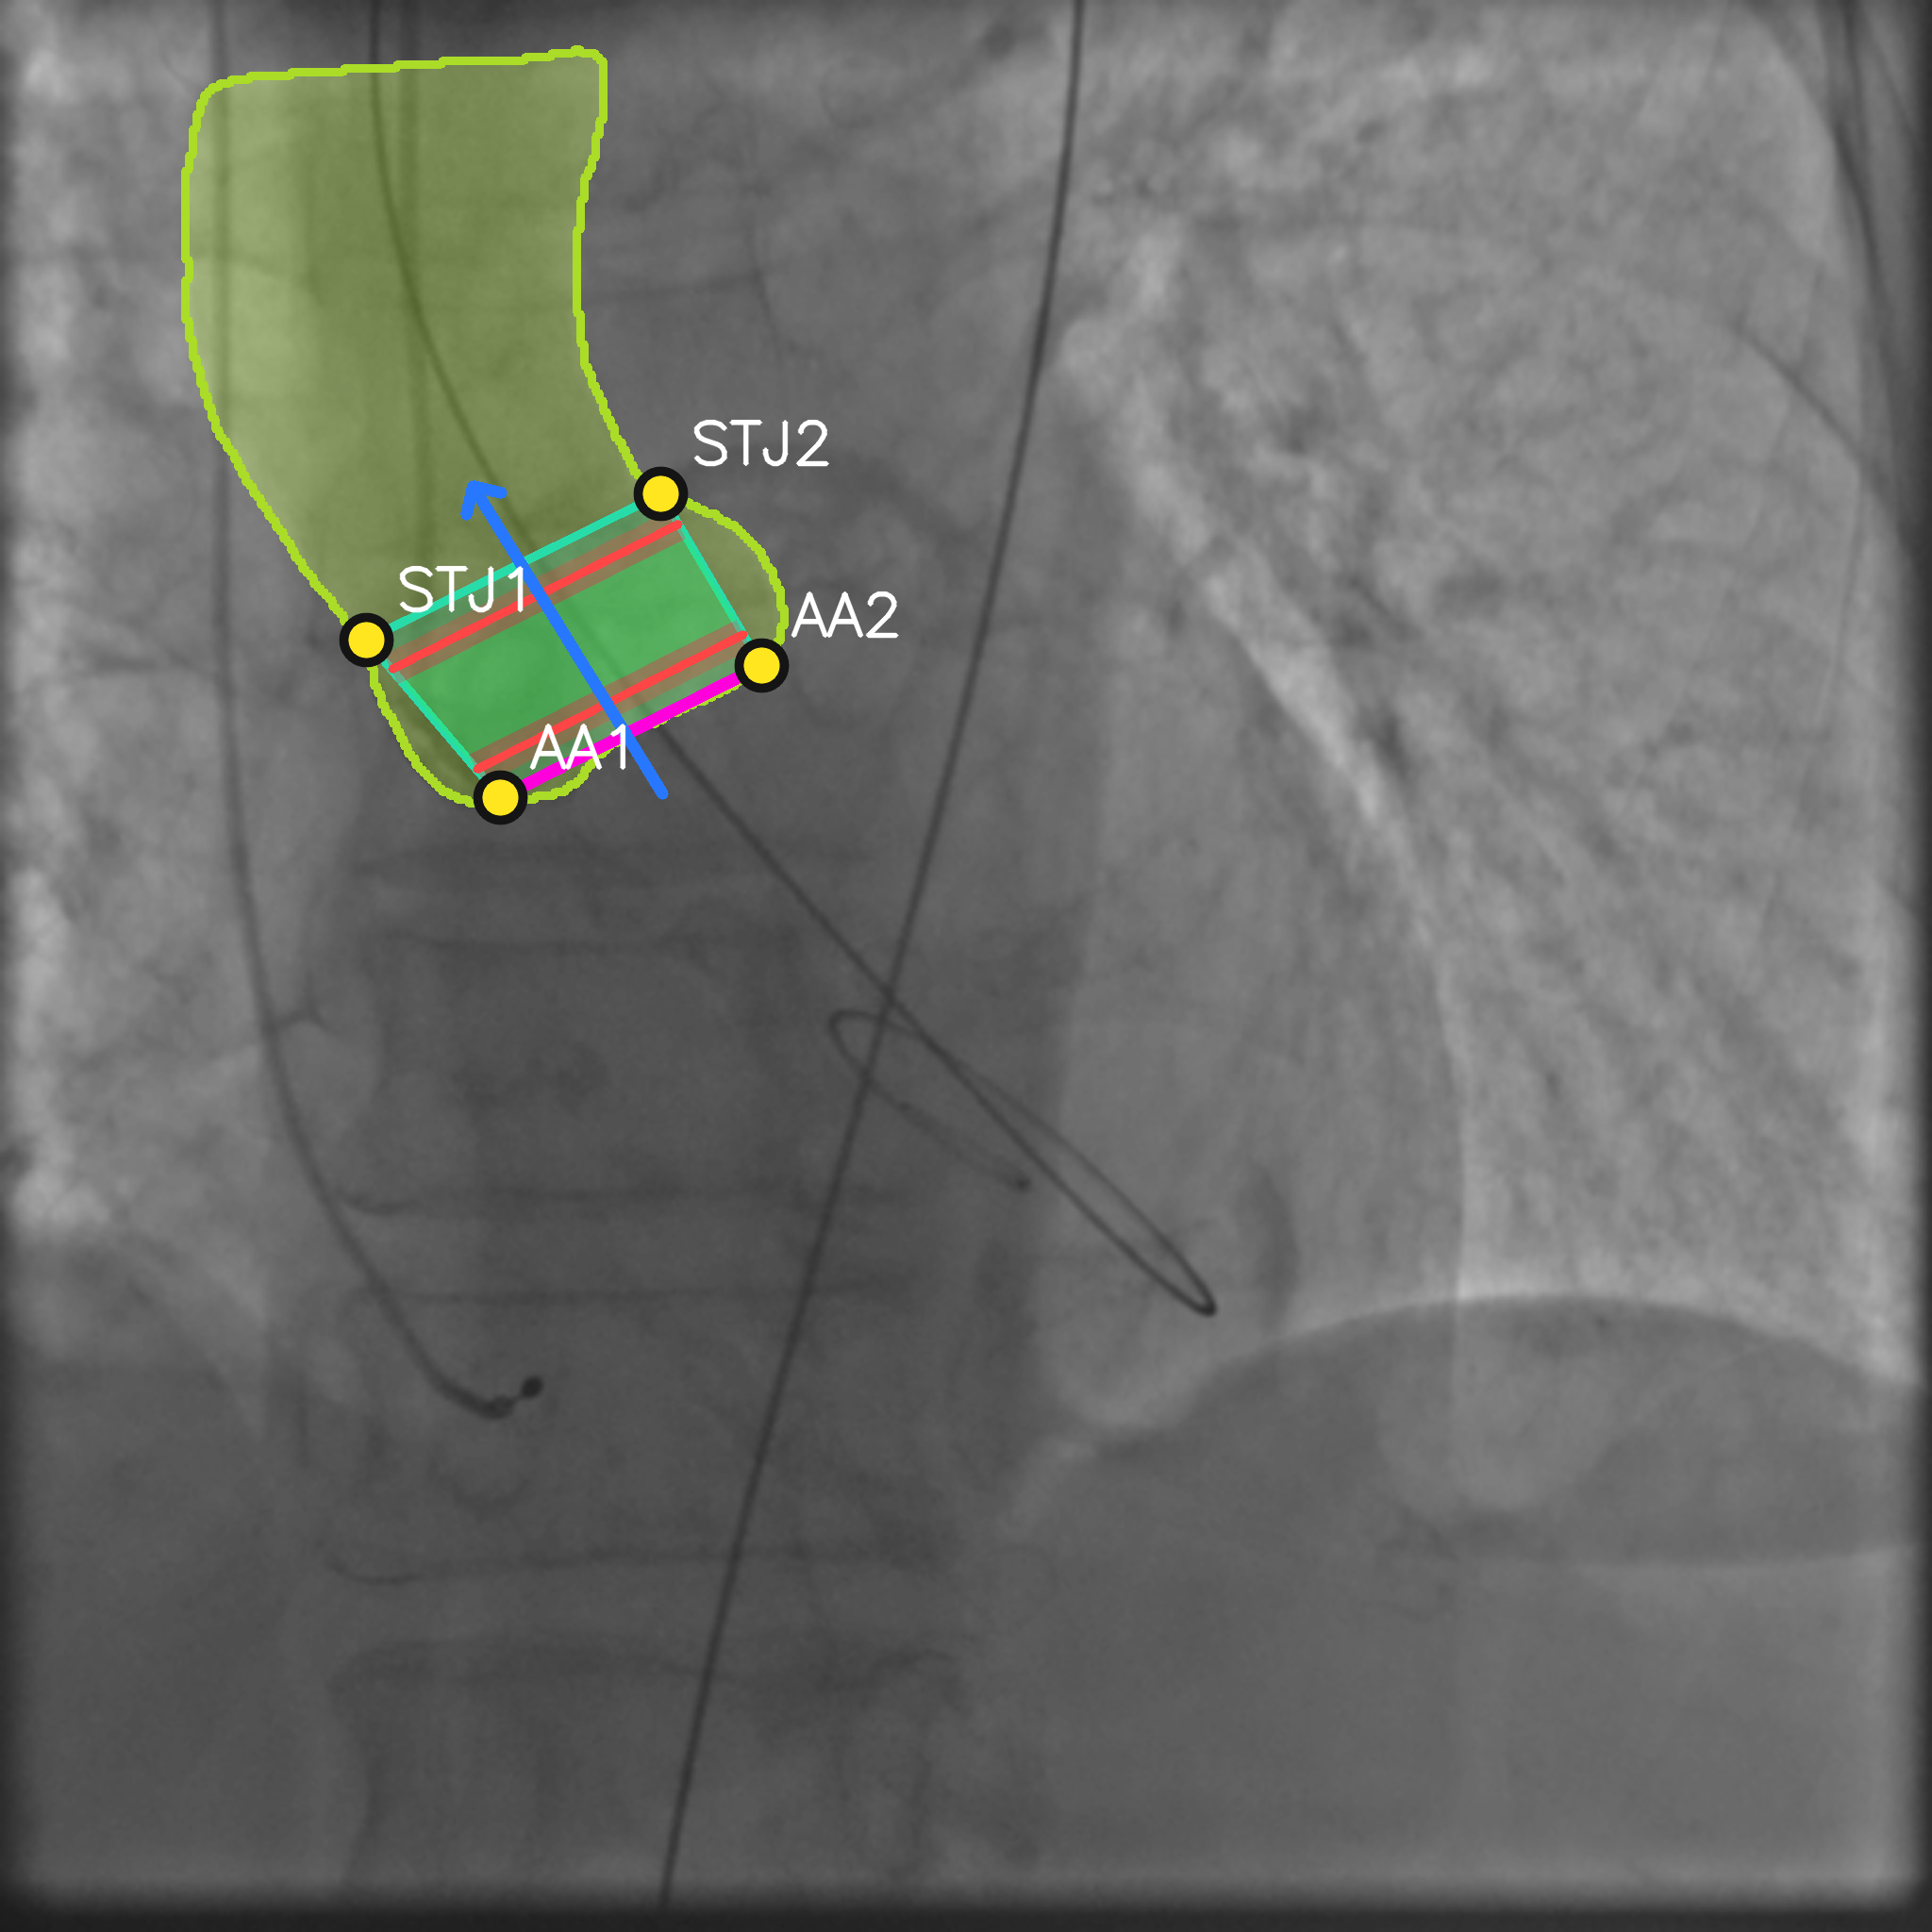
\includegraphics[width=0.48\textwidth]{figures/Figure_3b.png}}
\caption{Representative BAMNet predictions on intraoperative fluoroscopic frames. The yellow contour and semi-transparent green region denote the predicted aortic root mask. Yellow points correspond to the four predicted landmarks (AA1, AA2, STJ1, STJ2). The blue arrow indicates the estimated aortic axis, and the central geometric overlay illustrates the predicted implantation zone derived from the landmark configuration.}
\label{fig:bamnet_qualitative}
\end{figure}

\subsection{Patient-level 5-fold cross-validation}
\label{subsec:crossval}

To assess robustness, strict patient-level 5-fold cross-validation was performed. Across all five folds, the number of prediction failures remained zero, indicating stable behavior across different patient subsets. Mean performance across folds reached a Dice score of $0.916 \pm 0.011$, an IoU of $0.850 \pm 0.018$, a Surface Dice@4 mm of $0.845 \pm 0.031$, a median localization error of $7.64 \pm 0.33$ px, and a mean localization error of $10.02 \pm 0.17$ px.

The best segmentation quality was observed on fold 4, where Dice reached 0.93 and IoU 0.88. The smallest median localization error was obtained on fold 5 (7.32 px), whereas the smallest mean localization error was observed on fold 3 (9.91 px). Even the least favorable fold remained comparable to the others, supporting good inter-patient generalization.

\begin{table}[htbp]
\caption{Patient-level 5-fold cross-validation results for BAMNet.}
\label{tab:crossval}
\centering
\resizebox{\textwidth}{!}{%
\begin{tabular}{lcccccc}
\toprule
Fold & $n_{samples}$ & Dice & IoU & Surface Dice@4 mm & Median err. (px) & Mean err. (px) \\
\midrule
1 & 243 & 0.91 & 0.83 & 0.84 & 8.17 & 10.30 \\
2 & 250 & 0.91 & 0.83 & 0.81 & 7.59 & 9.92 \\
3 & 244 & 0.92 & 0.85 & 0.83 & 7.70 & 9.91 \\
4 & 249 & 0.93 & 0.88 & 0.89 & 7.45 & 10.05 \\
5 & 250 & 0.92 & 0.85 & 0.86 & 7.32 & 9.92 \\
Mean $\pm$ SD & 247.2 & $0.916 \pm 0.011$ & $0.850 \pm 0.018$ & $0.845 \pm 0.031$ & $7.64 \pm 0.33$ & $10.02 \pm 0.17$ \\
\bottomrule
\end{tabular}}
\end{table}

\subsection{Landmark-wise localization accuracy}

Landmark-specific analysis showed that AA1 was localized most accurately, with a mean error of $7.96 \pm 0.73$ px and a median error of $5.92 \pm 0.40$ px across folds. The most difficult point was AA2, for which the mean error reached $11.89 \pm 0.62$ px and the median error $9.95 \pm 1.37$ px. STJ1 and STJ2 showed intermediate performance, with STJ2 exhibiting greater inter-fold variability in mean error. Overall, all four landmarks were localized with clinically relevant precision, but the results suggest greater difficulty for landmarks affected by projection variability, incomplete contrast filling, and partial device overlap.

\begin{table}[htbp]
\caption{Landmark-wise localization accuracy aggregated over five folds.}
\label{tab:landmark_summary}
\centering
\resizebox{0.9\textwidth}{!}{%
\begin{tabular}{lccc}
\toprule
Landmark & Mean err. (px, mean $\pm$ SD) & Median err. (px, mean $\pm$ SD) & Std. err. (px, mean $\pm$ SD) \\
\midrule
AA1 & $7.96 \pm 0.73$ & $5.92 \pm 0.40$ & $7.66 \pm 1.61$ \\
AA2 & $11.89 \pm 0.62$ & $9.95 \pm 1.37$ & $8.60 \pm 1.00$ \\
STJ1 & $10.20 \pm 0.87$ & $7.66 \pm 0.14$ & $8.86 \pm 2.20$ \\
STJ2 & $10.02 \pm 1.46$ & $7.73 \pm 0.93$ & $8.28 \pm 2.01$ \\
\bottomrule
\end{tabular}}
\end{table}

The per-fold breakdown in Table~\ref{tab:landmark_folds} confirms this pattern. AA2 remained the most difficult landmark in terms of absolute error, whereas STJ2 showed the greatest between-fold variability in mean error. AA1 remained the most stable in median accuracy.

\begin{table}[htbp]
\caption{Per-fold landmark localization errors for BAMNet.}
\label{tab:landmark_folds}
\centering
\resizebox{\textwidth}{!}{%
\begin{tabular}{lcccc}
\toprule
Fold & AA1 mean / median (px) & AA2 mean / median (px) & STJ1 mean / median (px) & STJ2 mean / median (px) \\
\midrule
1 & 8.13 / 5.82 & 12.91 / 12.15 & 9.53 / 7.46 & 10.64 / 7.65 \\
2 & 6.81 / 5.39 & 11.43 / 9.18 & 9.16 / 7.57 & 12.27 / 9.31 \\
3 & 8.78 / 6.18 & 11.88 / 10.32 & 10.21 / 7.68 & 8.77 / 7.21 \\
4 & 8.24 / 6.43 & 11.86 / 9.47 & 11.20 / 7.77 & 8.89 / 6.93 \\
5 & 7.83 / 5.76 & 11.38 / 8.63 & 10.89 / 7.81 & 9.56 / 7.56 \\
\bottomrule
\end{tabular}}
\end{table}

\subsection{Overall interpretation}

Taken together, the results indicate that BAMNet is the most balanced model among the tested architectures. It remains competitive with strong segmentation baselines in Dice, IoU, and contour-sensitive metrics while also achieving lower mean landmark localization error than keypoint-only and detection-only approaches. Most importantly, this is achieved within a single model, without the need to chain separate segmentation and detection networks.

\section{Discussion}

This study introduced BAMNet, a multitask architecture specifically designed for simultaneous dense segmentation of the aortic root and localization of four anatomical landmarks directly on intraoperative fluoroscopic images acquired during TAVI. In patient-level 5-fold cross-validation, the model demonstrated stable performance, reaching Dice $0.916 \pm 0.011$, IoU $0.850 \pm 0.018$, Surface Dice@4 mm $0.845 \pm 0.031$, median localization error $7.64 \pm 0.33$ px, and mean localization error $10.02 \pm 0.17$ px. These results support the practicality of the approach for intraoperative visual guidance.

\subsection{Technical implications and architectural contribution}

The overall performance of BAMNet appears to arise not from a single isolated component but from the interaction of multiple design choices. The architecture combines an EfficientNet-V2 encoder, a modified MA-Net decoder, global spatial attention, a dedicated landmark heatmap head, an auxiliary boundary supervision pathway, and coordinate-aware feature modulation. Together, these components make it possible to maintain strong segmentation quality while also delivering clinically meaningful landmark coordinates.

The ablation study therefore focused on Position Attention in the decoder, Coordinate Attention in the landmark branch, deep-decoder feature fusion, boundary guidance and boundary loss, and the soft-argmax temperature schedule. This analysis assesses how global spatial context, coordinate-aware feature modulation, auxiliary boundary supervision, and heatmap-to-coordinate conversion affect the balance between segmentation quality and landmark localization accuracy. The contribution of each architectural component is summarized in Fig.~\ref{fig:ablation_summary}. From a deployment perspective, the main practical benefit is that BAMNet removes the need to run two separate models at inference time. The reported throughput of 63 FPS on an NVIDIA RTX 4070 is compatible with real-time fluoroscopic assistance.

\begin{figure}[htbp]
\centering
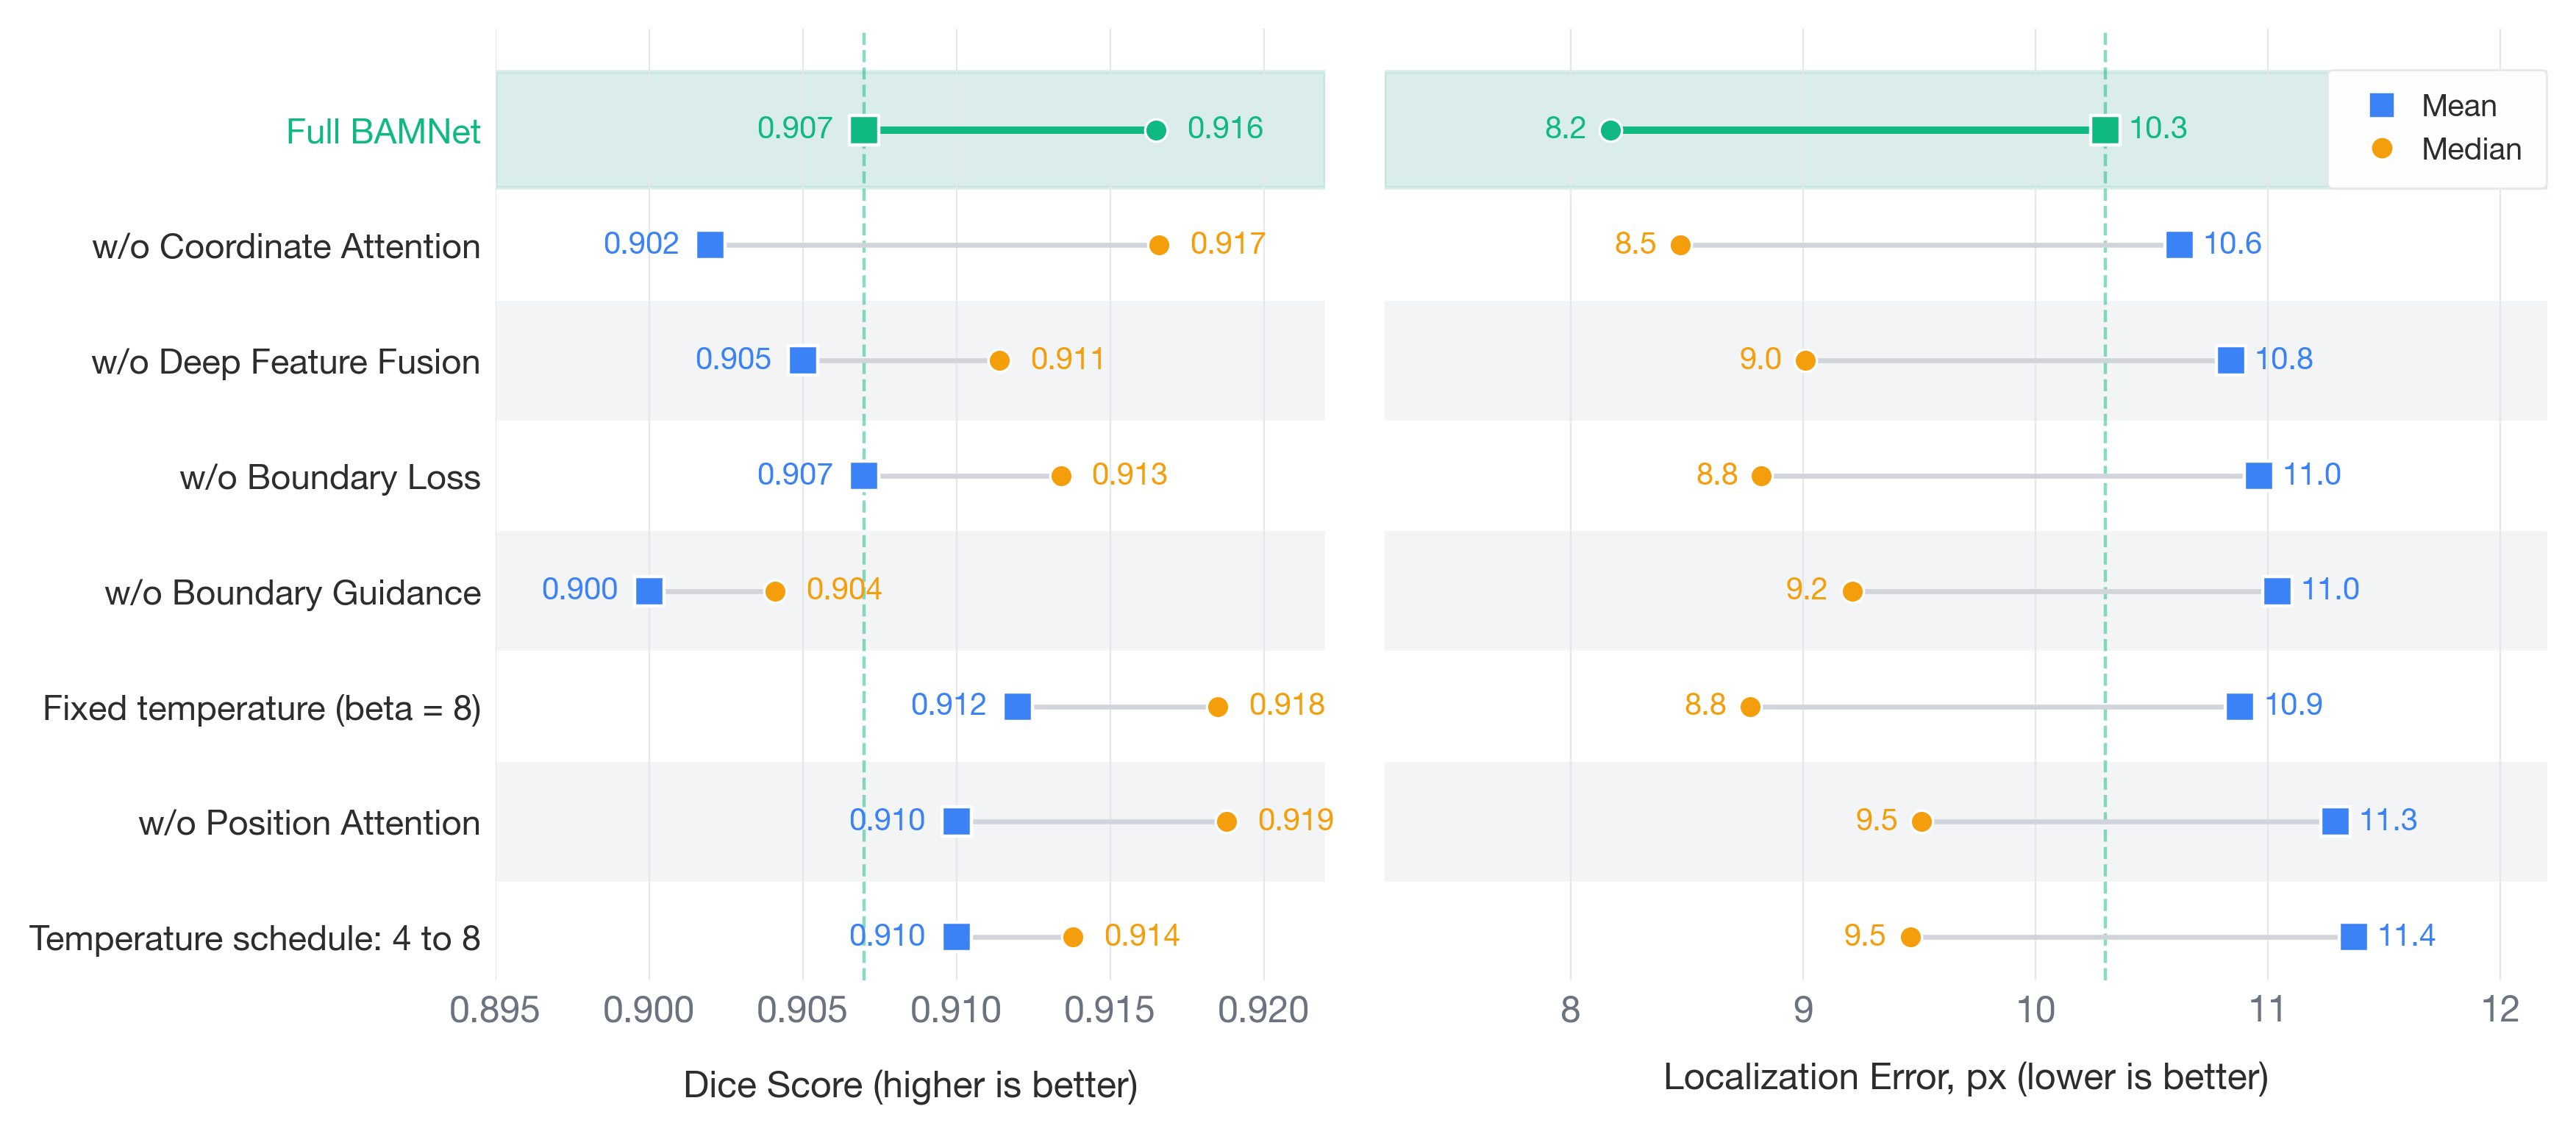
\includegraphics[width=\textwidth]{figures/Figure_4.png}
\caption{Summary of the BAMNet ablation study across the main architectural variants. The figure highlights how global spatial attention, coordinate-aware modulation, feature fusion, boundary-related supervision, and the soft-argmax configuration affect the balance between segmentation quality and landmark localization accuracy.}
\label{fig:ablation_summary}
\end{figure}

Numerical ablation results are summarized in Table~\ref{tab:ablation_results}. The variant with a fixed soft-argmax temperature of 8 achieved the highest Dice, IoU, and Surface Dice@4 mm, indicating particularly strong segmentation performance. However, the full BAMNet configuration yielded the lowest mean and median landmark localization errors together with the best PCK@10, and therefore provided the most balanced combination of segmentation quality and landmark localization accuracy. All ablation experiments were conducted on the fold-1 hold-out test set; cross-validated ablation was not performed due to computational cost.

\begin{table}[htbp]
\caption{Numerical results of the BAMNet ablation study across the main architectural variants. Evaluated on fold-1 fixed hold-out test set.}
\label{tab:ablation_results}
\centering
\resizebox{\textwidth}{!}{%
\begin{tabular}{lccccccc}
\toprule
Variant & Dice & IoU & Surface Dice@4 mm & Mean err. (px) & Median err. (px) & PCK@10 (\%) & FPS \\
\midrule
Full & 0.91 & 0.83 & 0.84 & \textbf{10.30} & \textbf{8.17} & \textbf{59.88} & 63 \\
No Pos Attn & 0.91 & 0.84 & 0.83 & 11.29 & 9.51 & 52.98 & \textbf{69} \\
No Coord Attn & 0.90 & 0.83 & 0.83 & 10.62 & 8.47 & 57.41 & 67 \\
No Fusion & 0.91 & 0.83 & 0.83 & 10.84 & 9.01 & 55.76 & 65 \\
No Bnd Guid & 0.90 & 0.82 & 0.82 & 11.04 & 9.21 & 53.70 & 66 \\
No Bnd Loss & 0.91 & 0.84 & 0.83 & 10.96 & 8.82 & 54.73 & 64 \\
Fixed 8 & \textbf{0.91} & \textbf{0.84} & \textbf{0.84} & 10.88 & 8.77 & 56.69 & 66 \\
Sched 4$\rightarrow$8 & 0.91 & 0.84 & 0.83 & 11.37 & 9.46 & 53.29 & 66 \\
\bottomrule
\end{tabular}}
\end{table}

\subsection{Clinical relevance}

Producing both an aortic root mask and key landmark coordinates in one pass has direct clinical relevance. One potential benefit is a reduced need for repeated contrast aortography. Although the present study did not measure the volume of contrast saved directly, continuous anatomical overlay on fluoroscopy could lower the number of repeat contrast series and may therefore be particularly useful in patients with chronic kidney disease or elevated risk of contrast-induced nephropathy \citep{dangas2020_tavi,yamamoto2021_tavi}.

A second important aspect is valve positioning accuracy. Even modest implantation-depth deviations are associated with paravalvular regurgitation, coronary obstruction, and conduction abnormalities requiring permanent pacing \citep{pibarot2021_pvl,jilaihawi2022_coronary,kammler2016_implantdepth}. In the present study, the median localization error on the validation set was 2.57 mm and the mean error was 3.22 mm. These values already approach a range that is potentially useful for visual assistance. The more conservative cross-validation results, with median and mean errors of $7.64 \pm 0.33$ px and $10.02 \pm 0.17$ px, still indicate reproducible performance suitable for stable anatomical overlay.

The third clinical implication concerns radiation burden. If the model reduces the need for additional angiographic runs, it may also reduce cumulative exposure for both the patient and the operating staff. Although radiation dose was not measured directly here, the task formulation is aligned with the ``as low as reasonably achievable'' principle and with the broader objective of safer intraoperative guidance.

\subsection{Toward robot-assisted and autonomous TAVI}

One of the most promising applications of BAMNet is robot-assisted or visually assisted TAVI. Such systems require more than segmentation alone: they need stable landmark coordinates that can support navigation, motion compensation, and possibly closed-loop control. This is why the multitask output of BAMNet is substantially more valuable than isolated segmentation in this context.

In patient-level 5-fold cross-validation, the median landmark localization error was $7.64 \pm 0.33$ px and the mean error was $10.02 \pm 0.17$ px, providing a realistic and more robust estimate of performance for clinically relevant scenarios. With the addition of temporal modeling, sequence-level filtering, and explicit compensation for cardiac and respiratory motion, further reductions in coordinate instability may be achievable. The fact that the model reasons over both local appearance and global spatial context may also make it more robust when the aortic root is partially obscured by the delivery system or catheters, which is precisely the setting where simple tracking or segmentation approaches often fail \citep{smits2025_autonomous,clinicaltrials_nct07152574}.

\subsection{Limitations}

This study has several limitations. First, despite the relatively large dataset of 2,925 images from 83 patients, the material remains single-center. External validation on data from other centers, fluoroscopy systems, and valve types is needed before broader generalization can be claimed. Second, all analysis was performed in a frame-wise setting; temporal consistency across neighboring frames was not studied. That limitation is particularly important for future integration into robotic systems.

Third, while the observed localization errors are promising for visual assistance, fully autonomous control would likely require higher precision together with predictable temporal stability. Finally, we have not yet performed a prospective clinical evaluation of the effect of BAMNet on procedure duration, contrast volume, radiation dose, or complication rates. The present results should therefore be interpreted as a technological proof of feasibility rather than definitive evidence of clinical benefit.

\subsection{Future directions}

Several natural extensions follow from the present work. The first is a move toward multi-frame modeling with temporal loss functions or recurrent or video architectures in order to stabilize landmark tracking throughout the cardiac cycle. A second direction is biplane fluoroscopy with 3D reconstruction of anatomical landmarks. A third is prospective clinical evaluation with explicit measurement of positioning accuracy, procedure duration, contrast use, and radiation exposure. Finally, an important translational direction is integration of BAMNet into a human-machine guidance loop for navigation and robot-assisted TAVI.

\section{Conclusion}

BoundaryAwareMANet (BAMNet) is a multitask deep learning architecture for simultaneous segmentation of the aortic root and localization of four key anatomical landmarks on intraoperative fluoroscopic images acquired during TAVI. Unlike single-task formulations, the proposed approach produces both a dense anatomical mask and a set of geometrically meaningful landmarks within one forward pass, making it especially attractive for intraoperative visual guidance.

In patient-level 5-fold cross-validation, BAMNet demonstrated stable performance with Dice $0.916 \pm 0.011$, IoU $0.850 \pm 0.018$, Surface Dice@4 mm $0.845 \pm 0.031$, median localization error $7.64 \pm 0.33$ px, and mean localization error $10.02 \pm 0.17$ px. These findings indicate that the model maintains high segmentation accuracy and reproducible landmark localization across different patient subsets, which is particularly important for clinically realistic assessment of generalization.

Thus, BAMNet can be regarded as a practical foundation for anatomical overlay during TAVI, a potential reduction in reliance on repeated contrast aortography, and the further development of semi-automated and robot-assisted valve implantation systems. Promising future directions include external multicenter validation, modeling of temporal consistency between neighboring frames, and integration of the model into a closed-loop intraoperative navigation pipeline.

\section*{Funding}

This work was supported by the Russian Science Foundation [grant number 24-19-00084].

\section*{Data availability}

All essential components of the study, including curated source code, data, and trained models, have been made publicly available:

\begin{itemize}
\item Source code: \url{https://github.com/Nikita75699/BAMNet}
\item Dataset: \url{https://doi.org/10.5281/zenodo.19219901}
\item Models: \url{https://doi.org/10.5281/zenodo.19295876}
\end{itemize}

\section*{Conflict of interest}

The authors declare that they have no known competing financial interests or personal relationships that could have appeared to influence the work reported in this paper.

\section*{Ethics statement}

Formal ethics committee approval was not required for this retrospective study because it used fully anonymized archival fluoroscopic images and did not involve access to directly identifiable patient information, in accordance with institutional policy and applicable local regulations. Informed consent to participate was waived because this study used fully anonymized retrospective archival imaging data and no patient-identifiable information was accessed. The manuscript contains only fully anonymized fluoroscopic images and does not include any information that could identify individual participants; consent for publication was therefore not required.

\section*{CRediT authorship contribution statement}

Nikita V. Laptev: Conceptualization, Data curation, Formal analysis, Investigation, Methodology, Software, Supervision, Validation, Visualization, Writing - original draft, Writing - review \& editing. Olga M. Gerget: Formal analysis, Investigation, Methodology, Software, Validation, Visualization, Writing - review \& editing. Julia K. Panteleeva: Data curation, Formal analysis, Visualization, Writing - review \& editing. Mikhail A. Chernyavsky: Data curation, Project administration, Resources, Supervision. Viacheslav V. Danilov: Methodology, Resources, Validation, Supervision, Writing - review \& editing.

\section*{Declaration of generative AI and AI-assisted technologies in the manuscript preparation process}

During the preparation of this work, the authors used OpenAI Codex to assist with manuscript structuring, language editing, and adaptation of the submission package to the target journal format. After using this tool, the authors reviewed and edited the content as needed and take full responsibility for the content of the published article.

\bibliographystyle{elsarticle-harv}
\bibliography{cmig}

\end{document}
